% Sostituisco i placeholder registrati con la specifica variabile per il documento corrente. Questa parte iniziale contiene intestazioni e templates.

% Modificare ad ogni modifica e documento
\newcommand{\documento}{\PdQ}
\newcommand{\nomedocumentofisico}{PianoDiQualifica 4\_0\_0.pdf}
\newcommand{\redazione}{\AN \\ & \NS \\ & \DS}
\newcommand{\verifica}{\AS}
\newcommand{\versione}{4.0.0}
\newcommand{\approvazione}{\DS}
\newcommand{\uso}{Esterno}
\newcommand{\destinateTo}{\TV, \\ & \RC, \\ & \IS}
\newcommand{\datacreazione}{20 Dicembre 2016}
\newcommand{\datamodifica}{11 Giugno 2017}
\newcommand{\stato}{Approvato}


%Abilitazione indice delle tabelle e figure
\def\TABELLE{false}
\def\FIGURE{false}

%Inclusione di layout e variabili (Non modificare)
%Stile e dimensione del documento
\documentclass[a4paper,11pt]{article}

%Pacchetti da importare
\usepackage{ifthen}
\usepackage[italian]{babel}
\usepackage[utf8]{inputenc}
\usepackage[T1]{fontenc}
\usepackage{float}
\usepackage{chapterbib}
\usepackage{graphicx}
\usepackage[a4paper,top=2.5cm,bottom=2.5cm,left=2.5cm,right=2.5cm]{geometry}
\usepackage[colorlinks=true, urlcolor=black, citecolor=black, linkcolor=black]{hyperref}
\usepackage{booktabs}
\usepackage{fancyhdr}
\usepackage{totpages}
\usepackage{tabularx, array}
\usepackage{dcolumn}
\usepackage{epstopdf}
\usepackage{booktabs}
\usepackage{fancyhdr}
\usepackage{longtable}
\usepackage{calc}
\usepackage{datatool}
\usepackage[bottom]{footmisc}
\usepackage{listings}
\usepackage{textcomp}
\usepackage{titlesec}
\usepackage{rotating}
\usepackage{multirow}
\usepackage{placeins}
\usepackage{color}
\usepackage[table,usenames,dvipsnames]{xcolor}
\usepackage{hyperref}
\usepackage{makecell}
\usepackage{breakurl}
\usepackage{hyperref}
\usepackage{multirow}
\usepackage{xcolor,colortbl}
\usepackage{afterpage}
\usepackage{mathtools}
\usepackage{verbatim} 
\usepackage[toc,page]{appendix}

%glossary code%
\usepackage[nonumberlist,xindy]{glossaries}

\newglossarystyle{myaltlistgroup}{%
	\setglossarystyle{altlistgroup}%
	\renewcommand*{\glsgroupheading}[1]{%
		
		\newpage
		\item\makebox[\linewidth]{\Large\textbf{\glsgetgrouptitle{##1}}}%
		\vspace*{-\baselineskip}%
		\item\makebox[\linewidth]{\hspace*{3cm}\hrulefill\hspace*{3cm}}%
	}%
}



%Stile fancy per il documento (Header e footer)
\pagestyle{fancy}
%Rimuovo l'indentazione
\setlength{\parindent}{0pt}

%Imposto l'intestazione
\lhead{\Large{\progetto} \\ \footnotesize{\documento}}
%Linea sotto l'intestazione
\renewcommand{\headrulewidth}{0.4pt} 

%Footer
\lfoot{\textit{\gruppoLink}\\ \footnotesize{\email}}
%Footer con numero romano per le prime pagine
\rfoot{\thepage}
\cfoot{}
%Linea sopra il footer
\renewcommand{\footrulewidth}{0.4pt}   

%Imposta il livello degli elenchi 
\setcounter{secnumdepth}{7}
\setcounter{tocdepth}{7}

%Paragrafi impostati come una sezione
\titleformat{\paragraph}{\normalfont\normalsize\bfseries}{\theparagraph}{1em}{}
\titlespacing*{\paragraph}{0pt}{3.25ex plus 1ex minus .2ex}{1.5ex plus .2ex}

\titleformat{\subparagraph}{\normalfont\normalsize\bfseries}{\thesubparagraph}{1em}{}
\titlespacing*{\subparagraph}{0pt}{3.25ex plus 1ex minus .2ex}{1.5ex plus .2ex}

\makeatletter
\newcounter{subsubparagraph}[subparagraph]
\renewcommand\thesubsubparagraph{
  \thesubparagraph.\@arabic\c@subsubparagraph}
\newcommand\subsubparagraph{
  \@startsection{subsubparagraph}
    {6}
    {\parindent}
    {3.25ex \@plus 1ex \@minus .2ex}
    {0.75em}
    {\normalfont\normalsize\bfseries}}
\newcommand\l@subsubparagraph{\@dottedtocline{6}{10em}{5.5em}} 
\newcommand{\subsubparagraphmark}[1]{}
\makeatother

\makeatletter
\newcounter{subsubsubparagraph}[subsubparagraph]
\renewcommand\thesubsubsubparagraph{
  \thesubsubparagraph.\@arabic\c@subsubsubparagraph}
\newcommand\subsubsubparagraph{
  \@startsection{subsubsubparagraph}
    {7}
    {\parindent}
    {3.25ex \@plus 1ex \@minus .2ex}
    {0.75em}
    {\normalfont\normalsize\bfseries}}
\newcommand\l@subsubsubparagraph{\@dottedtocline{7}{10em}{6.5em}}
\newcommand{\subsubsubparagraphmark}[1]{}
\makeatother

\renewcommand\appendixtocname{Appendice}
\renewcommand\appendixpagename{Appendice}
%Variabili generali
\newcommand{\progetto}{API Market}
\newcommand{\gruppo}{NetBreak}
\newcommand{\gruppoLink}{\href{https://git.io/v1Rgz}{NetBreak}}
\newcommand{\email}{netbreakswe@gmail.com}

%Variabili riguardanti i documenti
\newcommand{\AdR}{Analisi dei Requisiti}
\newcommand{\NdP}{Norme di Progetto}
\newcommand{\PdP}{Piano di Progetto}
\newcommand{\SdF}{Studio di Fattibilità}
\newcommand{\PdQ}{Piano di Qualifica}
\newcommand{\VE}{Verbale}
\newcommand{\ST}{Specifica Tecnica}
\newcommand{\DDP}{Definizione di Prodotto}
\newcommand{\MU}{Manuale Utente}
\newcommand{\G}{Glossario}
\newcommand{\LdP}{Lettera di Presentazione}

%Variabili per i membri del gruppo
\newcommand{\AS}{Andrea Scalabrin}
\newcommand{\NS}{Nicolò Scapin}
\newcommand{\AN}{Alberto Nicolè}
\newcommand{\DS}{Davide Scarparo}
\newcommand{\DAN}{Dan Serbanoiu}
\newcommand{\MC}{Marco Casagrande}

%Ruoli di progetto
\newcommand{\RdP}{Responsabile di Progetto}
\newcommand{\Res}{Responsabile}
\newcommand{\Amm}{Amministratore}
\newcommand{\Ver}{Verificatore}
\newcommand{\Prog}{Progettista}
\newcommand{\Progr}{Programmatore}
\newcommand{\Ana}{Analista}
\newcommand{\RdPs}{Responsabili di Progetto}
\newcommand{\Ress}{Responsabile}
\newcommand{\Amms}{Amministratori}
\newcommand{\Vers}{Verificatori}
\newcommand{\Progs}{Progettisti}
\newcommand{\Progrs}{Programmatori }
\newcommand{\Anas}{Analisti}

%Professori e proponente
\newcommand{\TV}{Prof. Tullio Vardanega}
\newcommand{\RC}{Prof. Riccardo Cardin}
\newcommand{\IS}{ItalianaSoftware S.r.l.}
\newcommand{\proponente}{ItalianaSoftware S.r.l.}

\newcommand{\diaryEntry}[5]{#2 & \emph{#4} & #3 & #5 & #1\\ \hline}

%Comando per una nuova riga nella tabella del changelog
\newcommand{\specialcell}[2][c]{%
	\begin{tabular}[#1]{@{}c@{}}#2\end{tabular}}

\renewcommand*\sectionmark[1]{\markboth{#1}{}}
\renewcommand*\subsectionmark[1]{\markright{#1}}

%Variabili per la fase di lavoro
\newcommand{\AR}{Analisi dei Requisiti}
\newcommand{\ARD}{Analisi dei Requisiti Dettagliata}
\newcommand{\PA}{Progettazione Architetturale}
\newcommand{\PD}{Progettazione Architetturale Dettagliata}
\newcommand{\CO}{Codifica}
\newcommand{\VV}{Verifica e Validazione}

%Variabili per le varie revisioni
\newcommand{\RR}{Revisione dei Requisiti}
\newcommand{\RP}{Revisione di Progettazione}
\newcommand{\RPMin}{Revisione di Progettazione Minima}
\newcommand{\RPMax}{Revisione di Progettazione Massima}
\newcommand{\RQ}{Revisione di Qualifica}
\newcommand{\RA}{Revisione di Accettazione}

\newcommand{\myincludegraphics}[2][]{%
	\setbox0=\hbox{\phantom{X}}%
	\vtop{
		\hbox{\phantom{X}}
		\vskip-\ht0
		\hbox{\includegraphics[#1]{#2}}}}

\renewcommand\footnoterule{\rule{\linewidth}{1pt}}

\newcommand{\nogloxy}[1]{#1} % comando da usare per evitare di metttere il mark del glossario
\newcommand{\gloxy}[1]{\emph{#1}$_G$}

\colorlet{punct}{red!60!black}
\definecolor{background}{HTML}{EEEEEE}
\definecolor{delim}{RGB}{20,105,176}
\colorlet{numb}{magenta!60!black}
\lstdefinelanguage{json}{
	basicstyle=\small\ttfamily,
	numbers=left,
	numberstyle=\scriptsize,
	stepnumber=1,
	numbersep=8pt,
	showstringspaces=false,
	breaklines=true,
	frame=lines,
	backgroundcolor=\color{background},
	literate=
	*{0}{{{\color{numb}0}}}{1}
	{1}{{{\color{numb}1}}}{1}
	{2}{{{\color{numb}2}}}{1}
	{3}{{{\color{numb}3}}}{1}
	{4}{{{\color{numb}4}}}{1}
	{5}{{{\color{numb}5}}}{1}
	{6}{{{\color{numb}6}}}{1}
	{7}{{{\color{numb}7}}}{1}
	{8}{{{\color{numb}8}}}{1}
	{9}{{{\color{numb}9}}}{1}
	{:}{{{\color{punct}{:}}}}{1}
	{,}{{{\color{punct}{,}}}}{1}
	{\{}{{{\color{delim}{\{}}}}{1}
	{\}}{{{\color{delim}{\}}}}}{1}
	{[}{{{\color{delim}{[}}}}{1}
	{]}{{{\color{delim}{]}}}}{1},
}
\lstset{language=json}
\lstset{literate=%
	{Ö}{{\"O}}1
	{Ä}{{\"A}}1
	{Ü}{{\"U}}1
	{é}{{\"s}}1
	{è}{{\"e}}1
	{à}{{\"a}}1
	{ö}{{\"o}}1
}

\newcommand{\impl}{\textcolor{Green}{Implementato}}
\newcommand{\implno}{\textcolor{Red}{Non Implementato}}
\newcommand\Tstrut{\rule{0pt}{3.2ex}}         % = `top' strut
\newcommand\Bstrut{\rule[-1.9ex]{0pt}{0pt}}   % = `bottom' strut
\definecolor{Gray}{gray}{0.85}
\usepackage[inline]{enumitem}

%Inclusione del changelog per il documento corrente

\newcommand{\modifiche}
{
	Approvazione del documento & \specialcell[t]{\AS\\\Res} & \specialcell[t]{2017-01-04\\1.0.0}
	\\
	\midrule
	Verifica del documento & \specialcell[t]{\DS \\ \AN \\\Vers} & \specialcell[t]{2016-12-13\\0.3.0}
	\\
	\midrule
	Modifiche minori sulla base della verifica & \specialcell[t]{\AS\\\Res} & \specialcell[t]{2016-12-10\\0.2.2}
	\\
	\midrule
	Modifiche alla sezione Capitolato C3 & \specialcell[t]{\NS\\\Ana} & \specialcell[t]{2016-12-08\\0.2.1}
	\\
	\midrule
	Verifica del documento & \specialcell[t]{\AN\\\Ver} & \specialcell[t]{2016-12-07\\0.2.0}
	\\
	\midrule
	Modifiche dei paragrafi sulla base della verifica & \specialcell[t]{\AS\\\Res} & \specialcell[t]{2016-12-06\\0.1.1}
	\\
	\midrule
	Verifica del documento & \specialcell[t]{\DS\\\Ver} & \specialcell[t]{2016-12-06\\0.1.0}
	\\
	\midrule
	Accorpati i documenti e modifiche minori & \specialcell[t]{\AS\\\Res} & \specialcell[t]{2016-12-05\\0.0.9}
	\\
	\midrule
	Stesura del capitolato C2 & \specialcell[t]{\MC\\\Ana} & \specialcell[t]{2016-12-03\\0.0.8}
	\\
	\midrule
	Stesura del capitolato C5 & \specialcell[t]{\AN\\\Ana} & \specialcell[t]{2016-12-03\\0.0.7}
	\\
	\midrule
	Stesura del capitolato C4 & \specialcell[t]{\DS\\\Ana} & \specialcell[t]{2016-12-03\\0.0.6}
	\\
	\midrule
	Stesura del capitolato C3 & \specialcell[t]{\NS\\\Ana} & \specialcell[t]{2016-12-03\\0.0.5}
	\\
	\midrule
	Stesura del capitolato C6 & \specialcell[t]{\DAN\\\Ana} & \specialcell[t]{2016-12-03\\0.0.4}
	\\
	\midrule	
	Stesura del capitolato C1 & \specialcell[t]{\AS\\\Ana} & \specialcell[t]{2016-12-02\\0.0.3}
	\\
	\midrule
	Stesura dell'introduzione & \specialcell[t]{\AS\\\Ana} & \specialcell[t]{2016-12-02\\0.0.2}
	\\
	\midrule
	Creato template documento & \specialcell[t]{\AS\\\Ana} & \specialcell[t]{2016-12-02\\0.0.1}
	\\	
}

%Imposto la profondità degli indici
\setcounter{secnumdepth}{7}
\setcounter{tocdepth}{7}


\begin{document}

%Inclusione del template per la homepage (Non modificare)
%Importante: Non modificare questo template
%Modificare il documento principale per cambiare le parti

\begin{center}


%Spaziatura verticale

\vspace{4em}

%Intestazione con nome del gruppo
\begin{center} 
	\begin{Huge}
		\textbf{\fontsize{15mm}{20mm}\selectfont \gruppoLink} 
	\end{Huge}
\end{center}

\begin{center}
	\begin{Large}
		\vspace{0.3em}
		\textbf{Progetto \progetto}
	\end{Large}
\end{center}

%Inclusione del logo

\includegraphics[keepaspectratio = true,width=6cm]{../../Template/img/LogoNetbreak.png}

%Prima pagina senza intestazione né piè di pagina	
\thispagestyle{empty}

%Le informazioni del documento sono ancorate a fine pagina
\vfill

%Nome del documento
\begin{Huge} \textbf{\documento} \end{Huge}

%Tabella centrale
\begin{center}
\large\textbf{Informazioni sul documento} \\ \vspace{2em}
\small
\begin{tabular}{r l}
	\textbf{Nome del documento} & \nomedocumentofisico \\
	\textbf{Data di creazione} & \datacreazione\\
	\textbf{Ultima modifica} & \datamodifica\\
	\textbf{Versione} & \versione\\
	\textbf{Stato} & \stato \\
	\textbf{Redatto da}	& \redazione\\
	\textbf{Verificato da}	& \verifica\\
	\textbf{Approvato da}	& \approvazione\\
	\textbf{Uso}  & \uso\\
	\textbf{Distribuzione} & \gruppo \\
	\textbf{Destinato a}  &  \destinateTo \\
	\textbf{Email di riferimento}  &  \email \\
\end{tabular}
\end{center}

\vspace{2em}

\normalsize
%Inclusione abstract
\textbf{Abstract\\} 
Questo documento contiene il \PdP\ relativo al prodotto \progetto\ determinato dal gruppo \gruppo.
\end{center}
\clearpage


%Registro delle modifiche e indice (Non modificare)
\pagenumbering{Roman}
\newpage
% Non modificare - Pagina di Layout per il changelog
\begin{center}
	\Large{\textbf{Changelog}}
	\\\vspace{0.5cm}
	\normalsize
	\begin{tabularx}{\textwidth}{cXcc}
		\textbf{Versione} & \textbf{Descrizione} & \textbf{Autore e Ruolo} & \textbf{Data}
		\\\toprule
		\modifiche
		\bottomrule
	\end{tabularx}
\end{center}

%Inserisce il link all'indice
%\addcontentsline{toc}{section}{Indice}
\newpage
\tableofcontents
\clearpage 

%Se è stata impostata a true la variabile per la lista delle tabelle, la mostra
\ifthenelse{\equal{\TABELLE}{true}} 
{\listoftables \newpage}{}

%Se è stata impostata a true la variabile per la lista delle figure, la mostra
\ifthenelse{\equal{\FIGURE}{true}}
{\listoffigures \newpage}{}

%Da qui comincia la numerazione normale
\pagenumbering{arabic}

%Imposta il formato di visualizzazione
\rfoot{\thepage~di~\pageref{TotPages}}

%Inclusione delle varie sezioni di contenuto
%Introduzione e contenuti di ogni tipo
\renewcommand*{\arraystretch}{1.6}


\newpage
\section{Introduzione}

\subsection{Scopo del documento}
Lo scopo del documento è quello di presentare una breve analisi di tutti i capitolati proposti, con le motivazioni che hanno portato il gruppo a scegliere il capitolato C1. Tutti i capitolati son stati analizzati con la medesima metodologia,  evidenziando le tecnologie necessarie, il dominio applicativo e le criticità, e dando un giudizio finale con le opinioni raccolte all'interno del gruppo.

\subsection{Scopo del prodotto}
Lo scopo del prodotto è la realizzazione di un \textit{API Market\ped{G}} per l'acquisto e la vendita di \textit{microservizi\ped{G}}. Il sistema offrirà la possibilità di registrare nuove \textit{API\ped{G}} per la vendita, permetterà la consultazione e la ricerca di API ai potenziali acquirenti, gestendo i permessi di accesso ed utilizzo tramite creazione e controllo di relative \textit{API key\ped{G}}. Il sistema, oltre alla web app stessa, sarà corredato di un \textit{API Gateway\ped{G}} per la gestione delle richieste e il controllo delle chiavi, e fornirà funzionalità avanzate di statistiche per il gestore della piattaforma e per i fornitori dei microservizi.

\subsection{Riferimenti normativi}
\begin{itemize}
	\item \textsc{NormeDiProgetto 2\_0\_0.pdf}
\end{itemize}

\subsection{Riferimenti informativi}
\begin{itemize}
	\item \textbf{Capitolato d'appalto C1:} APIM: An API Market Platform \\ \url{http://www.math.unipd.it/~tullio/IS-1/2016/Progetto/C1.pdf}
	\item \textbf{Capitolato d'appalto C2:} AtAVi: Accoglienza tramite Assistente Virtuale \\ \url{http://www.math.unipd.it/~tullio/IS-1/2016/Progetto/C2.pdf}
	\item \textbf{Capitolato d'appalto C3:} DeGeOP: A Designer and Geo-localizer Web App for Organizational Plants \\
	\url{http://www.math.unipd.it/~tullio/IS-1/2016/Progetto/C3.pdf}
	\item \textbf{Capitolato d'appalto C4:} eBread: applicazione di lettura per dislessici \\
	\url{http://www.math.unipd.it/~tullio/IS-1/2016/Progetto/C4.pdf}
	\item \textbf{Capitolato d'appalto C5:} Monolith: an interactive bubble provider \\
	\url{http://www.math.unipd.it/~tullio/IS-1/2016/Progetto/C5.pdf}
	\item \textbf{Capitolato d'appalto C6:} SWEDesigner: editor di diagrammi UML con generazione di codice \\
	\url{http://www.math.unipd.it/~tullio/IS-1/2016/Progetto/C6.pdf}
\end{itemize}

\subsection{Glossario}
Per semplificare la consultazione e disambiguare alcune terminologie tecniche, le voci indicate con la lettera \textit{G} a pedice sono descritte approfonditamente nel documento \textsc{Glossario 2\_0\_0.pdf} e specificate solo alla prima occorrenza all'interno del suddetto documento.
\newpage
\section{Qualità di prodotto}
	
Al fine di garantire una buona qualità di prodotto, il \textit{team\ped{G}} ha individuato dallo standard \textbf{\textit{ISO/IEC 9126\ped{G}}} le qualità che ritiene più importanti durante tutto il ciclo di vita del prodotto \progetto. Per ognuna delle qualità individuate, sono stati definiti obiettivi e metriche coerenti con i livelli di qualità dichiarati.

\begin{figure}[H]
	\centering
	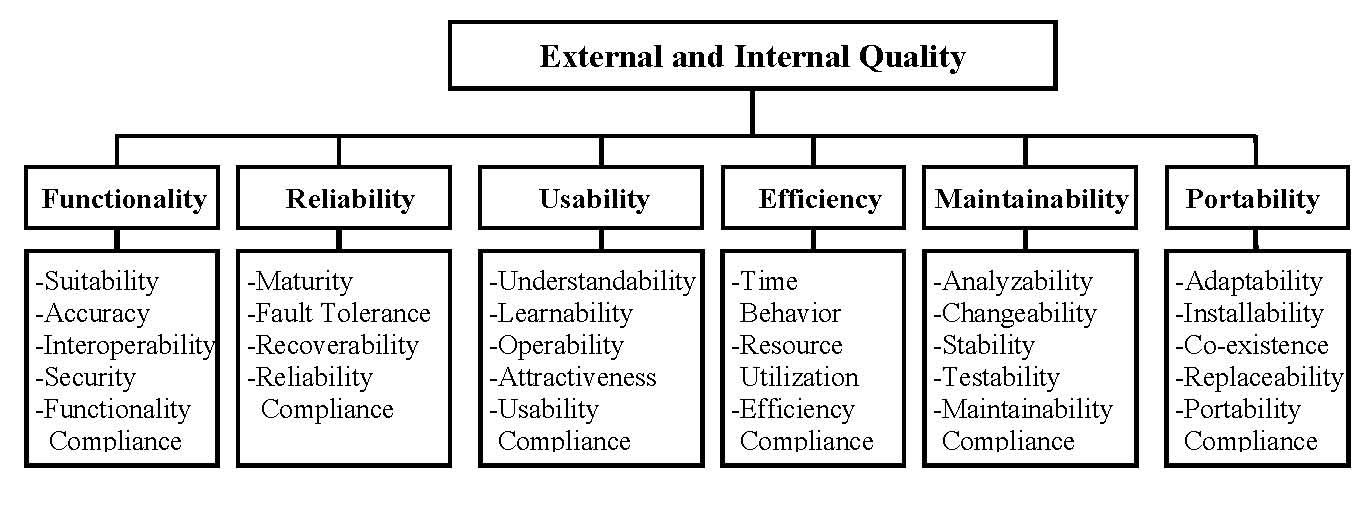
\includegraphics[scale=0.33]{includes/img/9126.png}
	\caption{Standard ISO/IEC 9126}
\end{figure}

Le \textbf{metriche interne} si applicano al software non eseguibile, come ad esempio le specifiche tecniche e il codice sorgente, durante i periodi di progettazione e codifica.
Esse sono specificate nella norma \textbf{\textit{ISO/IEC 9126-3\ped{G}}}.\\
Durante le fasi di sviluppo del software, i prodotti intermedi sono valutati tramite metriche interne che misurano le proprietà intrinseche del prodotto.
Le misure effettuate permettono di prevedere il livello di qualità esterna ed in uso del prodotto finale, in quanto gli attributi interni influenzano le caratteristiche esterne e quelle in uso.
Le metriche interne misurano attributi interni del software e forniscono indicazioni sulle caratteristiche esterne del prodotto finale, tramite l'analisi statica dei prodotti intermedi.
Le metriche interne si applicano anche alla documentazione del prodotto.\\
Le \textbf{metriche esterne} misurano i comportamenti del prodotto software rilevabili dai test, dall'operatività e dall'osservazione durante la su esecuzione, in funzione degli obiettivi stabiliti.
Esse sono specificate nella norma \textbf{\textit{ISO/IEC 9126-2\ped{G}}}.\\
Le metriche per la qualità di prodotto saranno identificate con la seguente sintassi:
\begin{center}
	\textbf{MPD}\_[\textit{Target}][[\textit{Id}]
\end{center}
dove:
\begin{itemize}
	\item \textbf{\textit{Target}} rappresenta la qualità di interesse della metrica e può assumere i valori:
	\begin{itemize}
		\item \textbf{\textit{F}} (Funzionalità);
		\item \textbf{\textit{A}} (Affidabilità);
		\item \textbf{\textit{U}} (Usabilità);
		\item \textbf{\textit{E}} (Efficienza);
		\item \textbf{\textit{M}} (Manutenibilità);
		\item \textbf{\textit{P}} (Portabilità);
	\end{itemize}
	\item \textbf{\textit{Id}} rappresenta il codice identificativo progressivo della metrica riguardante la qualità \textit{Target}. Questo indice viene fatto partire da 1 per ogni differente qualità.
\end{itemize}	

\subsection{Definizione degli obiettivi di qualità}

	\subsubsection{Funzionalità}
	Rappresenta la capacità del prodotto nel fornire le funzionalità richieste e soddisfare tutti i requisiti descritti nel documento \textsc{AnalisiDeiRequisiti 3\_0\_0.pdf}.
		
		\paragraph{Obiettivi}
			\begin{itemize}
				\item \textbf{Adeguatezza:} rappresenta la capacità di fornire un appropriato insieme di funzionalità che permettano agli utenti di svolgere determinati task e raggiungere gli obiettivi prefissati.
				\item \textbf{Accuratezza:} rappresenta la capacità di fornire i risultati e gli effetti attesi con il livello di precisione richiesta.
				\item \textbf{Sicurezza:} rappresenta la capacità di proteggere le informazioni ed i dati, in modo che persone o sistemi non autorizzati non possano accedervi.
			\end{itemize}
		
		\paragraph{Metriche}
			\subparagraph{Completezza delle funzioni sviluppate}
			\textbf{Id Metrica}: \hypertarget{MPDF1}{MPD\_F1}\\
			\textbf{Descrizione}: indica la percentuale di funzionalità sviluppate ritenute complete.
			
			\begin{itemize}
				\item \textbf{fun\ped{Compl}} = numero di funzioni ritenute complete
				\item \textbf{fun\ped{Tot}} = numero di funzioni totali
			\end{itemize}
			
		\begin{longtable}{>{\centering\arraybackslash}p{5cm}|>{\centering\arraybackslash}p{5cm} | >{\centering\arraybackslash}p{5cm}}
				\hline
				\rowcolor{Gray}
				\textbf{Metodo di calcolo} & \textbf{Range accettazione} & \textbf{Range ottimale} \\
				\hline
			     \begin{math}
			     \frac{fun\ped{Compl}}{fun\ped{Tot}}*100
			     \end{math} & [90,100] in [0,100]& [90,100] in [0,100] 
			\\
			\caption{Completezza delle funzioni sviluppate}
		\end{longtable}
			
			\subparagraph{Correttezza delle funzioni sviluppate}
			\textbf{Id Metrica}: \hypertarget{MPDF2}{MPD\_F2}\\
			\textbf{Descrizione}: indica la percentuale di funzionalità sviluppate ritenute corrette.
			
			\begin{itemize}
				\item \textbf{fun\ped{Corr}} = numero di funzioni ritenute corrette
				\item \textbf{fun\ped{Tot}} = numero di funzioni totali
			\end{itemize}
			
			\begin{longtable}{>{\centering\arraybackslash}p{5cm}|>{\centering\arraybackslash}p{5cm} | >{\centering\arraybackslash}p{5cm}}
					\hline
					\rowcolor{Gray}
					\textbf{Metodo di calcolo} & \textbf{Range accettazione} & \textbf{Range ottimale} \\
					\hline
					\begin{math}
					\frac{fun\ped{Corr}}{fun\ped{Tot}}*100
					\end{math} & 100 in [0,100]& 100 in [0,100] 
				
				\\
				\caption{Corretezza delle funzioni sviluppate}
			\end{longtable}
			
			\subparagraph{Accuratezza rispetto alle aspettative}
			\textbf{Id Metrica}: \hypertarget{MPDF3}{MPD\_F3}\\
			\textbf{Descrizione}: indica la percentuale di risultati conformi alle aspettative.
			
			\begin{itemize}
				\item \textbf{test\ped{Corr}} = numero di test ritenuti corretti
				\item \textbf{test\ped{Tot}} = numero di test totali
			\end{itemize}
			
			\begin{longtable}{>{\centering\arraybackslash}p{5cm}|>{\centering\arraybackslash}p{5cm} | >{\centering\arraybackslash}p{5cm}}
					\hline
					\rowcolor{Gray}
					\textbf{Metodo di calcolo} & \textbf{Range accettazione} & \textbf{Range ottimale} \\
					\hline
					\begin{math}
					\frac{test\ped{Corr}}{test\ped{Tot}}*100
					\end{math} & [90,100] in [0,100]& [95,100] in [0,100] 
				\\
				\caption{Accuratezza rispetto alle aspettative}
			\end{longtable}
						
			\subparagraph{Controllo degli accessi}
			\textbf{Id Metrica}: \hypertarget{MPDF4}{MPD\_F4}\\
			\textbf{Descrizione}: indica la percentuale di accessi corretti al sistema.
			
			\begin{itemize}
				\item \textbf{accessi\ped{Succ}} = numero di accessi controllati con successo dal sistema
				\item \textbf{accessi\ped{Tot}} = numero di accessi totali
			\end{itemize}
			
			\begin{longtable}{>{\centering\arraybackslash}p{5cm}|>{\centering\arraybackslash}p{5cm} | >{\centering\arraybackslash}p{5cm}}
					\hline
					\rowcolor{Gray}
					\textbf{Metodo di calcolo} & \textbf{Range accettazione} & \textbf{Range ottimale} \\
					\hline
					\begin{math}
					\frac{accessi\ped{Succ}}{accessi\ped{Tot}}*100
					\end{math} & [90,100] in [0,100]& 100 in [0,100] 
				\\
				\caption{Controllo degli accessi}
			\end{longtable}
			
	
	\subsubsection{Affidabilità}
	Rappresenta la capacità del prodotto software di mantenere il livello di prestazione, quando viene utilizzato in condizioni specificate.
		
		\paragraph{Obiettivi}
			\begin{itemize}
				\item \textbf{Maturità:} rappresenta la capacità di evitare che si verifichino errori o siano prodotti risultati non corretti in fase di esecuzione.
				\item \textbf{Tolleranza agli errori:} rappresenta la capacità di mantenere il livello di prestazioni in caso di errori nel software o di violazione nelle interfacce specificate.
			\end{itemize}
		
		\paragraph{Metriche}
			\subparagraph{Chiamate a microservizi corrette}
			\textbf{Id Metrica}: \hypertarget{MPDA1}{MPD\_A1}\\
			\textbf{Descrizione}: indica il numero di chiamate al microservizio j andate a buon fine.
			
			\begin{itemize}
				\item \textbf{num\ped{CF(MS(j))}} = numero di chiamate al microservizio j fallite o avvenute con successo, ma con t\ped{R(MS(j))} > t\ped{MR(MS(j))} + 0.3*t\ped{MR(MS(j))}, dove t\ped{R(MS(j))} = tempo di risposta del microservizio j e t\ped{MR(MS(j))} = tempo medio di risposta del microservizio j
				\item \textbf{num\ped{CT(MS(j))}} = numero totale di chiamate al microservizio j
			 
			\end{itemize}
			
			\begin{longtable}{>{\centering\arraybackslash}p{5cm}|>{\centering\arraybackslash}p{5cm} | >{\centering\arraybackslash}p{5cm}}
					\hline
					\rowcolor{Gray}
					\textbf{Metodo di calcolo} & \textbf{Range accettazione} & \textbf{Range ottimale} \\
					\hline
					\begin{math}
					\frac{num\ped{CF(MS(j))}}{num\ped{CT(MS(j))}}*100
					\end{math} & [90,100] in [0,100]& 100 in [0,100] 
				\\
				\caption{Chiamate a microservizi corrette}
			\end{longtable}
		
			\subparagraph{Copertura dei test}
			\textbf{Id Metrica}: \hypertarget{MPDA2}{MPD\_A2}\\
			\textbf{Descrizione}: indica il livello di copertura dei test.
			
			\begin{itemize}
				\item \textbf{test\ped{P}} = numero di test pianificati
				\item \textbf{test\ped{N}} = numero di test necessari a garantire la copertura richiesta o massima
			\end{itemize}
			
			\begin{longtable}{>{\centering\arraybackslash}p{5cm}|>{\centering\arraybackslash}p{5cm} | >{\centering\arraybackslash}p{5cm}}
					\hline
					\rowcolor{Gray}
					\textbf{Metodo di calcolo} & \textbf{Range accettazione} & \textbf{Range ottimale} \\
					\hline
					\begin{math}
					\frac{test\ped{P}}{test\ped{N}}*100
					\end{math} & [80,100] in [0,100] & 100 in [0,100] 
				\\
				\caption{Copertura dei test}
			\end{longtable}
			
			
			\subparagraph{Controllo dei guasti}
			\textbf{Id Metrica}: \hypertarget{MPDA3}{MPD\_A3}\\
			\textbf{Descrizione}: indica il livello di controllo dei guasti, attraverso il numero di condizioni di errore messe sotto controllo per evitare malfunzionamenti e/o guasti al prodotto.
			
			\begin{itemize}
				\item \textbf{num\ped{CEG}} = numero di condizioni d'errore gestite correttamente
				\item \textbf{num\ped{CEP}} = numero di condizioni d'errore possibili nel sistema
			\end{itemize}
			
			\begin{longtable}{>{\centering\arraybackslash}p{5cm}|>{\centering\arraybackslash}p{5cm} | >{\centering\arraybackslash}p{5cm}}
					\hline
					\rowcolor{Gray}
					\textbf{Metodo di calcolo} & \textbf{Range accettazione} & \textbf{Range ottimale} \\
					\hline
					\begin{math}
					\frac{num\ped{CEG}}{num\ped{CEP}}*100
					\end{math} & [80,100] in [0,100] & 100 in [0,100] 
				\\
				\caption{Controllo dei guasti}
			\end{longtable}
			
	
	\subsubsection{Usabilità}
	Rappresenta la capacità di un prodotto software di essere comprensibile, di poter essere studiato e di risultare attraente da parte di un utente sotto determinate condizioni.
	
		\paragraph{Obiettivi}
			\begin{itemize}
				\item \textbf{Comprensibilità:} rappresenta la capacità di permettere all'utente di capire le funzionalità del prodotto software e come poterle utilizzare con successo per svolgere particolari task in determinate condizioni di utilizzo.
				\item \textbf{Operabilità:} rappresenta la capacità di permettere all'utente di utilizzare e controllare il prodotto software.
				\item \textbf{Attrattività:} rappresenta la capacità di risultare piacevole per l'utente.
			\end{itemize}
		
		\paragraph{Metriche}
			\subparagraph{Comprensibilità delle funzionalità offerte}
			\textbf{Id Metrica}: \hypertarget{MPDU1}{MPD\_U1}\\
			\textbf{Descrizione}: indica la percentuale di funzioni comprensibili agli utenti.
			
				\begin{itemize}
				\item \textbf{num\ped{FC}} = numero di funzionalità comprensibili agli utenti
				\item \textbf{num\ped{FT}} = numero di funzionalità totali offerte
			\end{itemize}
			
			\begin{longtable}{>{\centering\arraybackslash}p{5cm}|>{\centering\arraybackslash}p{5cm} | >{\centering\arraybackslash}p{5cm}}
					\hline
					\rowcolor{Gray}
					\textbf{Metodo di calcolo} & \textbf{Range accettazione} & \textbf{Range ottimale} \\
					\hline
					\begin{math}
					\frac{num\ped{FC}}{num\ped{FT}}*100
					\end{math} & [80,100] in [0,100] & [90,100] in [0,100] 
				\\
				\caption{Comprensibilità delle funzionalità offerte}
			\end{longtable}
			
			\subparagraph{Controllo e monitoraggio delle operazioni}
			\textbf{Id Metrica}: \hypertarget{MPDU2}{MPD\_U2}\\
			\textbf{Descrizione}: indica la capacità del prodotto di monitorare lo stato delle operazioni eseguite.
			
				\begin{itemize}
				\item \textbf{num\ped{FC}} = numero di funzionalità con adeguato controllo e monitoraggio delle operazioni
				\item \textbf{num\ped{FCT}} = numero di funzionalità con controllo totali
			\end{itemize}
			
			
			\begin{longtable}{>{\centering\arraybackslash}p{5cm}|>{\centering\arraybackslash}p{5cm} | >{\centering\arraybackslash}p{5cm}}
					\hline
					\rowcolor{Gray}
					\textbf{Metodo di calcolo} & \textbf{Range accettazione} & \textbf{Range ottimale} \\
					\hline
					\begin{math}
					\frac{num\ped{FC}}{num\ped{FCT}}*100
					\end{math} & [80,100] in [0,100] & [90,100] in [0,100] 
				\\
				\caption{Controllo e monitoraggio delle operazioni}
			\end{longtable}
			
			\subparagraph{Qualità della messaggistica}
			\textbf{Id Metrica}: \hypertarget{MPDU3}{MPD\_U3}\\
			\textbf{Descrizione}: indica il grado di chiarezza, completezza e correttezza dei messaggi previsti rispetto alle diverse condizioni gestite dal prodotto (ad esempio, il completamento di una funzione, le condizioni di errore, le scelte da effettuare, etc.).
			
			\begin{itemize}
				\item \textbf{num\ped{MC}} = numero di messaggi che risultano chiari, completi e corretti
				\item \textbf{num\ped{MT}} = numero totale di messaggi previsti
			\end{itemize}
			
			\clearpage
			
			\begin{longtable}{>{\centering\arraybackslash}p{5cm}|>{\centering\arraybackslash}p{5cm} | >{\centering\arraybackslash}p{5cm}}
					\hline
					\rowcolor{Gray}
					\textbf{Metodo di calcolo} & \textbf{Range accettazione} & \textbf{Range ottimale} \\
					\hline
					\begin{math}
					\frac{num\ped{MC}}{num\ped{MT}}*100
					\end{math} & [70,100] in [0,100] & 100 in [0,100] 
				\\
				\caption{Qualità della messaggistica}
			\end{longtable}
	
	\subsubsection{Efficienza}
	Rappresenta la capacità di un prodotto software di realizzare le funzioni richieste nel minor tempo possibile ed utilizzando nel miglior modo le risorse necessarie.
		
		\paragraph{Obiettivi}
			\begin{itemize}
				\item \textbf{Comportamento rispetto al tempo:} rappresenta la capacità di fornire appropriati tempi di risposta, tempi di elaborazione e quantità di lavoro eseguendo le funzionalità previste.
				\item \textbf{Utilizzo delle risorse:} rappresenta la capacità di utilizzare un appropriato numero e tipo di risposte quando esegue le funzionalità previste.
			\end{itemize}
		
		\paragraph{Metriche}
			
			\subparagraph{Tempo di risposta}
			\textbf{Id Metrica}: \hypertarget{MPDE1}{MPD\_E1}\\
			\textbf{Descrizione}: indica il tempo medio che intercorre fra la richiesta di una determinata funzionalità e la restituzione del risultato all’utente. L'unità di misura scelta per esprimere il tempo è il \textit{secondo}.
			\begin{itemize}
				\item t\ped{i} = tempo trascorso
				fra la richiesta i di una funzionalità ed il completamento delle operazioni necessarie
				alla restituzione del risultato alla richiesta i
			\end{itemize}
		
		\begin{longtable}{>{\centering\arraybackslash}p{5cm}|>{\centering\arraybackslash}p{5cm} | >{\centering\arraybackslash}p{5cm}}
				\hline
				\rowcolor{Gray}
				\textbf{Metodo di calcolo} & \textbf{Range accettazione} & \textbf{Range ottimale} \\
				\hline
				\begin{math}
				\frac{\sum_{i=1}^{n}(t\ped{i})}{n} 
				\end{math} & [0,10] & [0,4]
			\\
			\caption{Tempo di risposta}
		\end{longtable}
			
			\iffalse
			\subparagraph{Tempo di risposta}
			Indica il tempo medio di risposta per una chiamata ad un microservizio j. La seguente formula viene usata per ridurre gli errori nel conteggio del valore medio su un insieme molto grande di dati.
			
			\begin{itemize}
				\item \textbf{MS(j)} = microservizio j
				\item \textbf{tI\ped{(i)(MS(j))}} = tempo di inizio della i-esima interazione col microservizio j
				\item \textbf{tF\ped{(i)(MS(j))}} = tempo di fine della i-esima interazione col microservizio j  
			\end{itemize}
			
			\begin{longtable}{>{\centering\arraybackslash}p{5cm}|>{\centering\arraybackslash}p{5cm} | >{\centering\arraybackslash}p{5cm}}
					\hline
					\rowcolor{Gray}
					\textbf{Metodo di calcolo} & \textbf{Range accettazione} & \textbf{Range ottimale} \\
					\hline
					\begin{math}
					\frac{1}{tI\ped{(i)(MS(j))}-tI\ped{(0)(MS(j))}}*(\sum_{1}^{n}(tF\ped{(2i)(MS(j))} - 4*tF\ped{(2i+1)(MS(j))} + tF\ped{(2i+2)(MS(j))}) 
					\end{math} con n = numero di interazioni col microservizio j &\begin{math}trisp(ms(j)) >= tmediorisp(ms(j)) + 0.3*tmediorisp(ms(j)) \end{math}& trisp(ms(j)) >= tmediorisp(ms(j)) + 0.05*tmediorisp(ms(j))
				\\
				\caption{Tempo di risposta}
			\end{longtable}
			\fi
	
	\subsubsection{Manutenibilità}
	Rappresenta la capacità di un prodotto software di essere modificato. Le modifiche possono includere correzioni o adattamenti del software a modifiche negli ambienti, nei requisiti e nelle specifiche funzionali.
	
		\paragraph{Obiettivi}
			\begin{itemize}
				\item \textbf{Analizzabilità:} rappresenta la capacità di poter effettuare la diagnosi sul software ed individuare le cause di errori o malfunzionamenti.
				\item \textbf{Modificabilità:} rappresenta la capacità di consentire lo sviluppo di modifiche al codice, alla progettazione e alla documentazione.
				\item \textbf{Stabilità:} rappresenta la capacità di evitare effetti non desiderati a seguito di modifiche al software.
				\item \textbf{Testabilità:} rappresenta la capacità di consentire la verifica e la validazione del software modificato, cioè di eseguire test.
			\end{itemize}
	
		\paragraph{Metriche}

			\subparagraph{Impatto delle modifiche}
			\textbf{Id Metrica}: \hypertarget{MPDM1}{MPD\_M1}\\
			\textbf{Descrizione}: indica la percentuale di modifiche effettuate in risposta a failure, le quali hanno portato all’introduzione di nuove failure in altre componenti del sistema.
			
			\begin{itemize}
				\item \textbf{num\ped{FRNF}} = numero di failure risolte con l’introduzione di nuove failure
				\item \textbf{num\ped{FR}} = numero di failure risolte
			\end{itemize}
			
			\begin{longtable}{>{\centering\arraybackslash}p{5cm}|>{\centering\arraybackslash}p{5cm} | >{\centering\arraybackslash}p{5cm}}
					\hline
					\rowcolor{Gray}
					\textbf{Metodo di calcolo} & \textbf{Range accettazione} & \textbf{Range ottimale} \\
					\hline
					\begin{math}
					\frac{num\ped{FRNF}}{num\ped{FR}}*100 
					\end{math} & [0,25] in [0,100] & [0,10] in [0,100]
				\\
				\caption{Impatto delle modifiche}
			\end{longtable}
		
	
	\subsubsection{Portabilità}
	Rappresenta la capacità di un prodotto software di poter essere trasportato da un ambiente ad un altro.
		
		\paragraph{Obiettivi}
			\begin{itemize}
				\item \textbf{Adattabilità:} rappresenta la capacità del prodotto di essere adattato a differenti ambienti, senza richiedere azioni specifiche diverse da quelle previste dal software per tali attività.
			\end{itemize}
		
		\paragraph{Metriche}
			\subparagraph{Supporto differenti versioni dei browser}
			\textbf{Id Metrica}: \hypertarget{MPDP1}{MPD\_P1}\\
			\textbf{Descrizione}: indica la percentuale di versioni dei browser supportate.
			
			\begin{itemize}
				\item \textbf{num\ped{VSupp}} = numero delle versioni dei browser supportati
				\item \textbf{num\ped{VTot}} = numero totale delle versioni che devono essere supportate
			\end{itemize}
			
			\begin{longtable}{>{\centering\arraybackslash}p{5cm}|>{\centering\arraybackslash}p{5cm} | >{\centering\arraybackslash}p{5cm}}
					\hline
					\rowcolor{Gray}
					\textbf{Metodo di calcolo} & \textbf{Range accettazione} & \textbf{Range ottimale} \\
					\hline
					\begin{math}
					\frac{num\ped{VSupp}}{num\ped{VTot}}*100
					\end{math}  & [90,100] in [0,100]  & 100 in [0,100] 
				\\
				\caption{Supporto differenti versioni dei browser}
			\end{longtable}
	
\newpage
\section{Qualità di processo}

	Per garantire la qualità del prodotto finale è necessario garantire la qualità dei processi necessari al suo completamento. A questo scopo, si è deciso di adottare lo standard \textbf{\textit{ISO/IEC 15504\ped{G}}}, denominato \textbf{\textit{SPICE\ped{G}}}.
	Esso si fonda sul principio che ogni processo deve essere controllato costantemente, in modo tale da rilevare possibili errori o debolezze, e correggerli prima che essi si diffondano, provocando un aumento del carico di lavoro e dello spreco di risorse.
	SPICE definisce sei livelli di maturità del processo:
	
	\begin{itemize}
		\item \textbf{Level 0 - Incomplete:} processo non ancora implementato o incapace di raggiungere i suoi obiettivi;
		\item \textbf{Level 1 - Performed:} processo messo in atto e capace di raggiungere i suoi obiettivi;
		\item \textbf{Level 2 - Managed:} processo eseguito sulla base di obiettivi ben definiti;
		\item \textbf{Level 3 - Established:} processo eseguito in base ai principi dell’ingegneria del software; 
		\item \textbf{Level 4 - Predictable:} processo attuato all’interno di limiti ben definiti;
		\item \textbf{Level 5 - Optimizing:} processo predicibile e capace di adattarsi per raggiungere obiettivi specifici e rilevanti;
	\end{itemize}
	
	Al fine di perseguire correttamente questo modello, è necessario adottare il principio \textbf{\textit{PDCA\ped{G}}}, il quale si compone delle seguenti quattro fasi:
	
	\begin{itemize}
		\item \textbf{Plan:} fase di pianificazione ed individuazione di obiettivi e processi, necessari allo scopo di raggiungere i risultati attesi;
		\item \textbf{Do:} fase di attuazione delle attività pianificate nella precedente fase Plan, e raccolta di dati sulla qualità ottenuta;
		\item \textbf{Check:} fase di verifica dove vengono confrontati i dati in uscita dalla fase Do con quelli pianificati nella fase Plan;
		\item \textbf{Act:} fase in cui si determinano le cause delle differenze fra risultati ottenuti e risultati attesi, in modo da individuare le azioni correttive da effettuare per ottenere un miglioramento della qualità.
	\end{itemize}

	\begin{figure}[H]
		\centering
		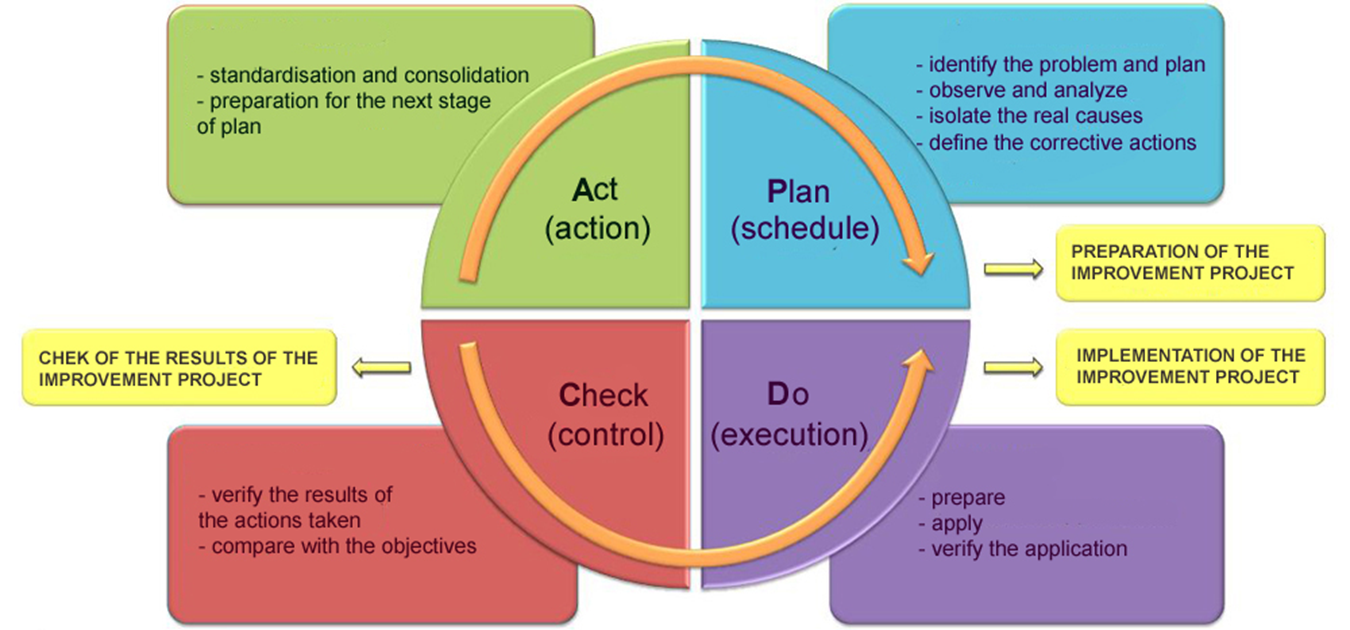
\includegraphics[scale=0.6]{includes/img/pdca.png}
		\caption{Principio PDCA.}
	\end{figure}

	Infine, il team ha individuato dallo standard \textbf{\textit{ISO/IEC 12207:2008\ped{G}}} i processi che ritiene più importanti durante tutto il ciclo di vita del prodotto, al fine di garantire una buona qualità di processo. Per ognuno di essi sono stati individuati obiettivi e metriche coerenti con i livelli di qualità perseguiti.
	
	\subsection{Infrastructure Management Process}
	Questo processo ha lo scopo di fornire, mantenere ed aggiornare l’infrastruttura ed i servizi necessari alla realizzazione del progetto, durante tutto il suo ciclo di vita. Il termine infrastruttura comprende: elementi hardware, software, metodi, strumenti, tecniche e standard impiegati nello sviluppo del prodotto.
	Essa sarà necessaria allo svolgimento del progetto e dovrà essere mantenuta costantemente aggiornata.
	L'utilizzo delle metriche scelte, permetterà di individuare eventuali errori all’interno degli strumenti utilizzati, la cui correzione permetterà di produrre dati corretti e coerenti.
		
		\subsubsection{Obiettivi}
		Per tutta la durata del progetto, l’infrastruttura impiegata nello sviluppo dovrà raggiungere i seguenti obiettivi:
		\begin{itemize}
			\item ogni procedura riguardante le attività svolte più frequentemente durante lo sviluppo del
			progetto, sarà descritta nel documento \textsc{NormeDiProgetto 2\_0\_0.pdf};
			\item ogni riferimento normativo ed informativo sarà completo di informazioni utili al proprio
			reperimento;
			\item la piattaforma \textit{NetBreakDB} sarà a disposizione di ogni componente del team, in caso di bisogno di accesso ai dati in essa contenuti;
		\end{itemize}
		\subsubsection{Metriche}
			\paragraph{Disponibilità \textit{NetBreakDB}}
			Indica la percentuale di disponibilità di utilizzo della piattaforma \textit{NetBreakDB}, rispetto alle richieste di accesso.
			
			\begin{itemize}
				\item \textbf{num\ped{AL}} = numero di accessi corretti alla pagina di login
				\item \textbf{num\ped{ALTot}} = numero totale delle richieste di accesso alla pagina di login inoltrate
			\end{itemize}
			
			\begin{table}[H]
				\begin{longtable}{>{\centering\arraybackslash}p{5cm}|>{\centering\arraybackslash}p{5cm} | >{\centering\arraybackslash}p{5cm}}
					\hline
					\rowcolor{Gray}
					\textbf{Metodo di calcolo} & \textbf{Range accettazione} & \textbf{Range ottimale} \\
					\hline
					\begin{math}
					\frac{num\ped{AL}}{num\ped{ALTot}}*100
					\end{math} & [80,100] in [0,100]  & 100 in [0,100] 
				\end{longtable}
				\caption{Disponibilità NetBreakDB}
			\end{table}
			
	\subsection{Project Planning, Assessment \& Control Process}
	Questo processo ha lo scopo di produrre dei piani di sviluppo per il progetto, che comprendano:
	\begin{itemize}
		\item la scelta del modello di ciclo di vita del prodotto;
		\item le descrizioni delle attività e dei compiti da svolgere;
		\item la pianificazione temporale del lavoro e dei costi da sostenere;
		\item l'allocazione di compiti e responsabilità;
		\item le misurazioni per rilevare lo stato del progetto, rispetto alle pianificazioni stilate.
	\end{itemize}
	Durante tutta l’attività di	progetto, sarà fondamentale mantenere aggiornata la pianificazione effettuata, in modo da essere sempre coerente con la situazione attuale. Nel caso in cui, in una fase di lavoro, venissero rilevati dei valori negativi, attraverso l'utilizzo delle metriche scelte Schedule Variance e Budget Variance, occorrerà compensare tali valori entro la fine dell’attività di progetto, al fine di evitare di eccedere le ore di lavoro totali e, di conseguenza, il preventivo dei costi finale indicato nella pianificazione contenuta nel documento \textsc{PianoDiProgetto 2\_0\_0.pdf}.
		\subsubsection{Obiettivi}
		L’intero sviluppo del progetto dovrà seguire la pianificazione prodotta:
		\begin{itemize}
			\item ogni componente dovrà svolgere e portare a termine l'attività assegnatagli, svolgendo tutti i compiti nei quali è stata suddivisa e facendo attenzione a rispettare le scadenze fissate;
			\item il costo necessario allo svolgimento di un'attività non dovrà eccedere la somma
			preventivata.
		\end{itemize}
		\subsubsection{Metriche}
			\paragraph{Schedule Variance}
			Indica se si è o meno in linea con la pianificazione temporale delle attività nella baseline.
			Se si ottiene un valore maggiore di 0, significa che il team è in anticipo, se si ottiene 0, significa che il team ha rispettato la pianificazione, altrimenti, in caso di valore negativo, significa che il team è in ritardo.
			
				\begin{itemize}
				\item \textbf{att\ped{Compl}} = attività completate ad un certo momento
				\item \textbf{att\ped{PCompl}} = attività che, secondo la pianificazione, dovrebbero essere state completate a quel momento
			\end{itemize}
			
			\begin{table}[H]
				\begin{longtable}{>{\centering\arraybackslash}p{5cm}|>{\centering\arraybackslash}p{5cm} | >{\centering\arraybackslash}p{5cm}}
					\hline
					\rowcolor{Gray}
					\textbf{Metodo di calcolo} & \textbf{Range accettazione} & \textbf{Range ottimale} \\
					\hline
					\begin{math}
					{att\ped{Compl} - att\ped{PCompl}}
					\end{math}  &  \begin{math}\geq{0} \end{math}  &  \begin{math}\geq{0} \end{math} 
				\end{longtable}
				\caption{Schedule Variance}
			\end{table}
		
		\paragraph{Budget Variance}
		Indica se la spesa sostenuta alla data corrente è superiore o inferiore a quella preventivata in sede di pianificazione.
		Un valore positivo indica che si è speso meno di quanto inizialmente previsto, altrimenti significa che si è speso più della somma preventivata.
		
		\begin{itemize}
			\item \textbf{costo\ped{Plan}} = costo pianificato per realizzare le attività di progetto alla data corrente
			\item \textbf{costo\ped{Eff}} = costo effettivamente sostenuto alla data corrente
		\end{itemize}
		
		\begin{table}[H]
			\begin{longtable}{>{\centering\arraybackslash}p{5cm}|>{\centering\arraybackslash}p{5cm} | >{\centering\arraybackslash}p{5cm}}
				\hline
				\rowcolor{Gray}
				\textbf{Metodo di calcolo} & \textbf{Range accettazione} & \textbf{Range ottimale} \\
				\hline
				\begin{math}
				{costo\ped{Plan} - costo\ped{Eff}}
				\end{math} & \begin{math}\geq{0} \end{math}  & \begin{math}\geq{0} \end{math}
			\end{longtable}
			\caption{Budget Variance}
		\end{table}
		
	\subsection{Risk Management Process}
	Questo processo ha l'obiettivo di identificare, analizzare, trattare e monitorare in modo continuo i rischi che possono insorgere durante l’intera attività di progetto.
	Il livello di probabilità dei rischi analizzati dovrà essere costantemente monitorato. Nel caso si manifestasse un rischio, a qualsiasi livello di pericolosità, il team dovrà attuare le contromisure previste, al fine di mitigarne gli effetti ed evitare un incremento del livello di pericolosità.
		\subsubsection{Obiettivi}
		Il team dovrà gestire correttamente i rischi:
		\begin{itemize}
			\item all’inizio dell’attività di progetto, verranno individuati i principali fattori di rischio riguardanti l’organizzazione delle attività;
			\item all’inizio di ogni attività, l’analisi dei rischi potrà portare all’individuazione di nuovi specifici rischi per ognuna di esse;
			\item i rischi analizzati che si manifesteranno, verranno trattati secondo le strategie descritte, così da controllarne l'impatto.
		\end{itemize}
		\subsubsection{Metriche}
			\paragraph{Rischi non preventivati}
			Indicatore che evidenzia i rischi non preventivati.
			
			\begin{itemize}
				\item \textbf{risk\ped{NP}} = contatore che viene incrementato nel momento in cui si manifesta un rischio non individuato nell’attività di analisi dei rischi
			\end{itemize}
			
			\begin{table}[H]
				\begin{longtable}{>{\centering\arraybackslash}p{5cm}|>{\centering\arraybackslash}p{5cm} | >{\centering\arraybackslash}p{5cm}}
					\hline
					\rowcolor{Gray}
					\textbf{Metodo di calcolo} & \textbf{Range accettazione} & \textbf{Range ottimale} \\
					\hline
					risk\ped{NP} & [0,5]  & 0 
				\end{longtable}
				\caption{Rischi non preventivati}
			\end{table}			
	
	\subsection{System/Software Requirements Analysis Process}
	Questo processo ha lo scopo di creare un insieme di requisiti tecnici, a partire dall'insieme di requisiti individuati dalle fonti, in modo che diventi la linea guida nella progettazione del prodotto.
	Ogni requisito individuato dovrà essere inserito correttamente nella piattaforma \textit{NetBreakDB}, la quale si occuperà di effettuare il tracciamento delle fonti dalle quali derivano i requisiti, delle modifiche effettuate e della loro implementazione nel prodotto.
		
		\subsubsection{Obiettivi}
		I requisiti identificati dovranno essere gestiti in modo da raggiungere i seguenti obiettivi:
		\begin{itemize}
			\item per ogni requisito dovrà essere possibile indicare dei test, da effettuare per verificarne il soddisfacimento da parte del prodotto;
			\item nessun requisito dovrà risultare ambiguo;
			\item tutti i requisiti che il prodotto andrà a soddisfare, saranno stati precedentemente approvati dal proponente.
		\end{itemize}
		
		\subsubsection{Metriche}
			
			\paragraph{Adempimento requisiti obbligatori}
			Indica la percentuale di requisiti obbligatori soddisfatti dal prodotto.
			
			\begin{itemize}
				\item \textbf{num\ped{ROS}} = numero di requisiti obbligatori soddisfatti
				\item \textbf{num\ped{ROI}} = numero di requisiti obbligatori identificati 
			\end{itemize}
			
			\begin{table}[H]
				\begin{longtable}{>{\centering\arraybackslash}p{5cm}|>{\centering\arraybackslash}p{5cm} | >{\centering\arraybackslash}p{5cm}}
					\hline
					\rowcolor{Gray}
					\textbf{Metodo di calcolo} & \textbf{Range accettazione} & \textbf{Range ottimale} \\
					\hline
					\begin{math}
					\frac{num\ped{ROS}}{num\ped{ROI}}*100
					\end{math}  & 100 in [0,100]  & 100 in [0,100]
				\end{longtable}
				\caption{Adempimento requisiti obbligatori}
			\end{table}
			
	\subsection{System/Software Architectural Design Process}
	Il processo si pone come obiettivo quello di identificare una corrispondenza fra requisiti di sistema ed elementi del sistema. Nel corso dell’attività di Progettazione, sia ad alto livello che di dettaglio, le componenti verranno inserite nella piattaforma \textit{NetBreakDB}. Essa si occuperà di effettuare i tracciamenti fra le componenti e i requisiti che soddisfano, ed inoltre, il tracciamento tra le relazioni presenti e le varie componenti.
		
		\subsubsection{Obiettivi}
		Durante lo svolgimento delle attività previste da questo processo, il team punterà a definire
		un’architettura adatta agli scopi del progetto:
		\begin{itemize}
			\item ogni componente progettato come parte del sistema risulterà essere necessario per il funzionamento del prodotto e, quindi, costantemente tracciabile ai requisiti che soddisfa;
			\item il sistema dovrà presentare basso accoppiamento ed alta coesione;
			\item ogni componente dovrà essere progettato puntando su incapsulamento, modularizzazione
			e riuso di codice.
		\end{itemize}
		
		\subsubsection{Metriche}
			\paragraph{Fan In}
			In riferimento ad un modulo software, misura quanti altri moduli lo utilizzano durante la loro esecuzione.
			Tale indicazione consente di stabilire il livello di riuso implementato.
			
			\begin{itemize}
				\item \textbf{FI} = contatore che viene incrementato nel momento in cui viene individuato un modulo che, durante la sua esecuzione, chiama il modulo in oggetto
			\end{itemize}
			
			\begin{table}[H]
				\begin{longtable}{>{\centering\arraybackslash}p{5cm}|>{\centering\arraybackslash}p{5cm} | >{\centering\arraybackslash}p{5cm}}
					\hline
					\rowcolor{Gray}
					\textbf{Metodo di calcolo} & \textbf{Range accettazione} & \textbf{Range ottimale} \\
					\hline
					FI & \begin{math}\geq{0} \end{math}   & \begin{math}\geq{3} \end{math} 
				\end{longtable}
				\caption{Fan In}
			\end{table}
			
			\paragraph{Fan Out}
			In riferimento ad un modulo software, misura quanti moduli vengono utilizzati durante la
			sua esecuzione.
			Tale indicazione consente di stabilire il livello di accoppiamento implementato.
			
			\begin{itemize}
				\item \textbf{FO} = contatore che viene incrementato nel momento in cui viene individuato un modulo utilizzato dal modulo in oggetto, durante la sua esecuzione
			\end{itemize}
	
		\begin{table}[H]
		\begin{longtable}{>{\centering\arraybackslash}p{5cm}|>{\centering\arraybackslash}p{5cm} | >{\centering\arraybackslash}p{5cm}}
			\hline
			\rowcolor{Gray}
			\textbf{Metodo di calcolo} & \textbf{Range accettazione} & \textbf{Range ottimale} \\
			\hline
			FO & [0,5] & [0,1]
		\end{longtable}
		\caption{Fan Out}
		\end{table}			
	
	\subsection{Software Architectural Design Process}
	Lo scopo del processo è fornire una progettazione di minimo del prodotto che andrà a soddisfare i requisiti individuati.
	Tutte le attività presenti in questo processo portano alla produzione del documento Specifica Tecnica.
		
		\subsubsection{Obiettivi}
			\begin{itemize}
				\item fornire un'architettura ad alto livello del prodotto software, in grado di soddisfare i requisiti individuati;
				\item definire le interfacce interne ed esterne per ogni componente individuato;
				\item progettare uno schema ad alto livello del database. 
			\end{itemize}
	
	\subsection{Software Detailed Design Process}
	Lo scopo del processo è fornire una progettazione dettagliata del prodotto che andrà ad implementare i requisiti individuati.
	Sarà necessario effettuare un’analisi dettagliata delle componenti individuate durante l'attività di progettazione
	architetturale, suddividendole in unità che siano facilmente codificabili e testabili.
		
		\subsubsection{Obiettivi}
		Le attività svolte dovranno raggiungere i seguenti obiettivi:
		\begin{itemize}
			\item il livello di dettaglio della progettazione dovrà indicare tutti i metodi, con i relativi parametri e campi dati, forniti da ciascuna classe;
			\item la struttura a basso livello dell’architettura e le relazioni fra le varie unità software concepite saranno esposte nel documento \textit{Definizione di Prodotto}, il quale definirà esattamente cosa implementare;
		\end{itemize}
		
		\subsubsection{Metriche}
			
			\paragraph{Numero di metodi per classe}
			Indica il numero di metodi definiti in una classe.
			Un valore molto alto potrebbe indicare una
			non buona decomposizione delle funzionalità a livello logico.
			
			\begin{itemize}
				\item \textbf{num\ped{MetCl}} = contatore che indica il numero di metodi definiti in una classe
			\end{itemize}
			
			\begin{table}[H]
				\begin{longtable}{>{\centering\arraybackslash}p{5cm}|>{\centering\arraybackslash}p{5cm} | >{\centering\arraybackslash}p{5cm}}
					\hline
					\rowcolor{Gray}
					\textbf{Metodo di calcolo} & \textbf{Range accettazione} & \textbf{Range ottimale} \\
					\hline
					num\ped{MetCl} & [1,10] & [1,5]
				\end{longtable}
				\caption{Numero di metodi per classe}
			\end{table}
			
		
			\paragraph{Numero di parametri per metodo}
			Indica il numero di parametri passati ad un metodo.
			Un valore molto alto potrebbe indicare un'eccessiva complessità del metodo, il quale potrebbe non essere sufficientemente scomposto in sotto-metodi.
			
			\begin{itemize}
				\item \textbf{num\ped{Par}} = contatore che indica il numero di parametri passati ad un metodo
			\end{itemize}
			
			\begin{table}[H]
				\begin{longtable}{>{\centering\arraybackslash}p{5cm}|>{\centering\arraybackslash}p{5cm} | >{\centering\arraybackslash}p{5cm}}
					\hline
					\rowcolor{Gray}
					\textbf{Metodo di calcolo} & \textbf{Range accettazione} & \textbf{Range ottimale} \\
					\hline
					num\ped{Par} & [0,8] & [0,4]
				\end{longtable}
				\caption{Numero parametri per metodo}
			\end{table}
			
			\paragraph{Numero di attributi per classe}
			Indica il numero di attributi di una classe.
			Un valore molto alto potrebbe suggerire la necessità di suddividere tale classe in più classi differenti correlate tra loro.
			
			\begin{itemize}
				\item \textbf{num\ped{AttrCl}} = contatore che indica il numero di attributi per una determinata classe
			\end{itemize}
			
			\begin{table}[H]
				\begin{longtable}{>{\centering\arraybackslash}p{5cm}|>{\centering\arraybackslash}p{5cm} | >{\centering\arraybackslash}p{5cm}}
					\hline
					\rowcolor{Gray}
					\textbf{Metodo di calcolo} & \textbf{Range accettazione} & \textbf{Range ottimale} \\
					\hline
					num\ped{AttrCl} & [0,12] & [2,8]
				\end{longtable}
				\caption{Numero di attributi per classe}
			\end{table}
			
			
	\subsection{Software Construction Process}
	Questo processo definisce le principali attività volte alla produzione di unità software eseguibili, che
	rispettino quanto prodotto durante la progettazione.
	Nell’attività di Codifica, il \textit{\Progr} dovrà semplicemente attenersi a quanto indicato nel documento \textit{Definizione di Prodotto}. Inoltre, sarà necessario procedere con la codifica dei test individuati in sede di progettazione, al fine di verificare il corretto funzionamento delle varie unità prodotte.
		
		\subsubsection{Obiettivi}
		Affinchè le unità software prodotte risultino di qualità, il team ha individuato i seguenti obiettivi:
		\begin{itemize}
			\item l’implementazione delle classi e dei metodi definiti in progettazione dovrà produrre codice a bassa complessità, in modo da facilitare l'attività di test;
			\item l’uso di costrutti e tecniche che creano sdoppiamenti del flusso di esecuzione verrà attuato solo se strettamente necessario;
			\item il codice prodotto dovrà risultare facilmente manutenibile;
			\item il codice prodotto risulterà privo di elementi inutilizzati.
		\end{itemize}
		
		\subsubsection{Metriche}
			
			\paragraph{Complessità Ciclomatica}
			Indica la complessità di funzioni, moduli, metodi o classi di un programma, misurando il numero
			di cammini linearmente indipendenti attraverso il grafo di controllo di flusso.
			Alti valori di complessità ciclomatica implicano una ridotta manutenibilità del codice; viceversa, bassi valori potrebbero determinare una scarsa efficienza dei metodi.
			
				\begin{itemize}
				\item \textbf{num\ped{Archi}} = numero di archi del grafo di controllo di flusso
				\item \textbf{num\ped{Nodi}} = numero di nodi del grafo di controllo di flusso
			\end{itemize}
			
			\begin{table}[H]
				\begin{longtable}{>{\centering\arraybackslash}p{5cm}|>{\centering\arraybackslash}p{5cm} | >{\centering\arraybackslash}p{5cm}}
					\hline
					\rowcolor{Gray}
					\textbf{Metodo di calcolo} & \textbf{Range accettazione} & \textbf{Range ottimale} \\
					\hline
					num\ped{Archi} - num\ped{Nodi} + 2 & [3,12] & [1,10]
				\end{longtable}
				\caption{Complessità Ciclomatica}
			\end{table}
			
			
			\paragraph{Numero di livelli di annidamento}
			Indica il numero di funzioni o procedure chiamate all’interno di un metodo.
			Un valore elevato implica un’alta complessità ed un basso livello di astrazione del codice.
			
			\begin{itemize}
				\item \textbf{nesting} = contatore che indica il numero di chiamate a funzioni o procedure
				presenti all’interno di un metodo
			\end{itemize}
			
			\begin{table}[H]
				\begin{longtable}{>{\centering\arraybackslash}p{5cm}|>{\centering\arraybackslash}p{5cm} | >{\centering\arraybackslash}p{5cm}}
					\hline
					\rowcolor{Gray}
					\textbf{Metodo di calcolo} & \textbf{Range accettazione} & \textbf{Range ottimale} \\
					\hline
					nesting & [1,8] & [1,4]
				\end{longtable}
				\caption{Numero di livelli di annidamento}
			\end{table}
		
			\paragraph{Linee di commento}
			Indica la percentuale di linee di commento presenti all’interno del codice sorgente; la loro presenza
			permette una più semplice comprensione ed un maggior livello di manutenibilità di quanto
			prodotto.
			
			\begin{itemize}
				\item \textbf{num\ped{LComm}} = numero di linee di commento presenti nel codice
				\item \textbf{num\ped{SLOC}} = numero di Source Line Of Code totali prodotte 
			\end{itemize}
			
			\begin{table}[H]
				\begin{longtable}{>{\centering\arraybackslash}p{5cm}|>{\centering\arraybackslash}p{5cm} | >{\centering\arraybackslash}p{5cm}}
					\hline
					\rowcolor{Gray}
					\textbf{Metodo di calcolo} & \textbf{Range accettazione} & \textbf{Range ottimale} \\
					\hline
					\begin{math}
					\frac{num\ped{LComm}}{num\ped{SLOC}}*100
					\end{math}  & [20,100] in [0,100] & [35,100] in [0,100]
				\end{longtable}
				\caption{Linee di commento}
			\end{table}
	
	\subsection{System/Software Qualification Testing Process}
	Lo scopo del processo è quello di assicurare che ogni requisito individuato sia stato implementato nel prodotto.
	Sarà indispensabile rendere il più possibile automatizzata l’esecuzione dei test di sistema, in modo tale che la loro esecuzione non richieda costi e tempi eccessivi, e  allo stesso tempo sia possibile eseguirne un numero sufficiente a garantire un’ottima copertura
	dei requisiti.
		
		\subsubsection{Obiettivi}
		Durante lo svolgimento delle attività di test, il team dovrà perseguire i seguenti obiettivi:
			\begin{itemize}
				\item le attività di test previste dal processo verranno svolte su un sistema le cui componenti sono verificate e correttamente integrate fra loro;
				\item il sistema dovrà implementare e soddisfare tutti i requisiti obbligatori individuati durante l'attività di analisi dei requisiti.
			\end{itemize}
		
		\subsubsection{Metriche}
			\paragraph{Test di Unità}
			Indica la percentuale di test di unità eseguiti.
			
			\begin{itemize}
				\item \textbf{num\ped{TUE}} = numero di test di unità eseguiti
				\item \textbf{num\ped{TUP}} = numero di test di unità panificati
			\end{itemize}
			
			\begin{table}[H]
				\begin{longtable}{>{\centering\arraybackslash}p{5cm}|>{\centering\arraybackslash}p{5cm} | >{\centering\arraybackslash}p{5cm}}
					\hline
					\rowcolor{Gray}
					\textbf{Metodo di calcolo} & \textbf{Range accettazione} & \textbf{Range ottimale} \\
					\hline
					\begin{math}
					\frac{num\ped{TUE}}{num\ped{TUP}}*100
					\end{math} & [95,100] in [0,100] & 100 in [0,100]
				\end{longtable}
				\caption{Test di Unità}
			\end{table}
		
			\paragraph{Test di Integrazione}
			Indica la percentuale di test di integrazione eseguiti.
			
			\begin{itemize}
				\item \textbf{num\ped{TIE}} = numero di test di integrazione eseguiti
				\item \textbf{num\ped{TIP}} = numero di test di integrazione pianificati
			\end{itemize}
			
			\begin{table}[H]
				\begin{longtable}{>{\centering\arraybackslash}p{5cm}|>{\centering\arraybackslash}p{5cm} | >{\centering\arraybackslash}p{5cm}}
					\hline
					\rowcolor{Gray}
					\textbf{Metodo di calcolo} & \textbf{Range accettazione} & \textbf{Range ottimale} \\
					\hline
					\begin{math}
					\frac{num\ped{TIE}}{num\ped{TIP}}*100
					\end{math} & [65,100] in [0, 100] & [75,100] in [0,100]
				\end{longtable}
				\caption{Test di Integrazione}
			\end{table}
			
			\paragraph{Test di Sistema}
			Indica la percentuale di test di sistema eseguiti.
			
			\begin{itemize}
				\item \textbf{num\ped{TSE}} = numero di test di sistema eseguiti
				\item \textbf{num\ped{TSP}} = numero di test di sistema pianificati
			\end{itemize}
			
			\begin{table}[H]
				\begin{longtable}{>{\centering\arraybackslash}p{5cm}|>{\centering\arraybackslash}p{5cm} | >{\centering\arraybackslash}p{5cm}}
					\hline
					\rowcolor{Gray}
					\textbf{Metodo di calcolo} & \textbf{Range accettazione} & \textbf{Range ottimale} \\
					\hline
					\begin{math}
					\frac{num\ped{TSE}}{num\ped{TSP}}*100
					\end{math} & [75,100] in [0,100] & [85,100] in [0,100]
				\end{longtable}
				\caption{Test di Sistema}
			\end{table}
			
			\paragraph{Test superati}
			Indica la percentuale di test totali superati.
			
			\begin{itemize}
				\item \textbf{num\ped{TS}} = numero di test superati
				\item \textbf{num\ped{TE}} = numero di test eseguiti
			\end{itemize}
			
			\begin{table}[H]
				\begin{longtable}{>{\centering\arraybackslash}p{5cm}|>{\centering\arraybackslash}p{5cm} | >{\centering\arraybackslash}p{5cm}}
					\hline
					\rowcolor{Gray}
					\textbf{Metodo di calcolo} & \textbf{Range accettazione} & \textbf{Range ottimale} \\
					\hline
					\begin{math}
					\frac{num\ped{TS}}{num\ped{TE}}*100
					\end{math}  & [95,100] in [0,100] & 100 in [0,100]
				\end{longtable}
				\caption{Test superati}
			\end{table}
			
	\subsection{Software Documentation Management Process}
	Questo processo ha l'obiettivo di produrre e manutenere le informazioni sul software prodotte dai processi
	attuati, attraverso un'opportuna documentazione.
	Ogni documento sarà dotato di:
		\begin{itemize}
			\item numero di versione;
			\item changelog.
		\end{itemize}
	Queste informazioni consentono di tenere traccia di ogni azione effettuata sul documento in oggetto.
		
		\subsubsection{Obiettivi}
		Il processo di documentazione dovrà perseguire le seguenti direttive:
			\begin{itemize}
				\item la documentazione prodotta dovrà essere chiara e comprensibile a tutti gli stakeholder e sarà resa disponibile alle parti interessate per la consultazione;
				\item ogni forma di ambiguità sul significato di un termine utilizzato verrà eliminata grazie al documento \textsc{Glossario 2\_0\_0.pdf};
				\item la documentazione prodotta sarà sempre aggiornata ed allineata allo stato attuale del
				processo di sviluppo del prodotto.
			\end{itemize}
		
		\subsubsection{Metriche}
			
			\paragraph{Indice Gulpease}
			L'indice Gulpease è un indice di leggibilità di un testo tarato sulla lingua italiana.
			Rispetto ad altri indici, questo ha il vantaggio di utilizzare la lunghezza delle parole in lettere, anziché in sillabe, semplificandone il calcolo automatico. L'indice Gulpease considera due variabili linguistiche:
			\begin{itemize}
				\item la lunghezza della parola;
				\item la lunghezza della frase, rispetto al numero delle lettere.
			\end{itemize}
			I risultati sono compresi tra 0 e 100, dove il valore 100 indica la leggibilità più alta, mentre il valore 0 la leggibilità più bassa.
			
			\begin{itemize}
				\item \textbf{num\ped{Frasi}} = numero di frasi
				\item \textbf{num\ped{Lettere}} = numero di lettere
				\item \textbf{num\ped{Parole}} = numero di parole
			\end{itemize}
			
			\begin{table}[H]
				\begin{longtable}{>{\centering\arraybackslash}p{5cm}|>{\centering\arraybackslash}p{5cm} | >{\centering\arraybackslash}p{5cm}}
					\hline
					\rowcolor{Gray}
					\textbf{Metodo di calcolo} & \textbf{Range accettazione} & \textbf{Range ottimale} \\
					\hline
					\begin{math}89+
					\frac{300*num\ped{Frasi}-10*num\ped{Lettere}}{num\ped{Parole}}
					\end{math} & [40,100] in [0,100] & [60,100] in [0,100]
				\end{longtable}
				\caption{Indice Gulpease}
			\end{table}
			
	
	\subsection{Software Verification Process}
	Questo processo ha lo scopo di verificare se un qualsiasi elemento del sistema soddisfa in modo esaustivo i requisiti ad esso associati.
	Durante le varie attività di revisione della documentazione, gli errori più frequenti rilevati verranno
	riportati in un documento apposito, in modo tale da velocizzare le successive attività di \textit{Inspection}.
	Inoltre, per ogni test effettuato verrà tenuto il tracciamento del suo esito.
		
		\subsubsection{Obiettivi}
		Al fine di garantire qualità durante questo processo, il team ha fissato i seguenti obiettivi:
		\begin{itemize}
			\item la documentazione verrà verificata attraverso la tecnica \textit{Inspection}, poiché permette di risparmiare tempo e costi;
			\item i test dinamici effettuati sui vari elementi saranno automatizzati il più possibile;
			\item i test dinamici effettuati sui vari elementi del software copriranno una grande parte dei possibili casi d'uso.
		\end{itemize}
		
		\subsubsection{Metriche}
			\paragraph{Code Coverage}
			Indica la percentuale di istruzioni che sono eseguite durante i test.
			Un alto valore di questo indice implica un'alta probabilità che le componenti testate abbiano una ridotta quantità di errori.
			Per ottenere un indice basso è necessario che l'implementazione dei metodi sia molto semplice, in modo da non richiedere alcuna attività di testing. Ad esempio, i metodi getter e setter.
			
			\begin{itemize}
				\item \textbf{num\ped{LM}} = numero di linee di codice monitorato dai test
				\item \textbf{num\ped{LI}} = numero di linee di codice implementate nel software
			\end{itemize}
			
			\begin{table}[H]
				\begin{longtable}{>{\centering\arraybackslash}p{5cm}|>{\centering\arraybackslash}p{5cm} | >{\centering\arraybackslash}p{5cm}}
					\hline
					\rowcolor{Gray}
					\textbf{Metodo di calcolo} & \textbf{Range accettazione} & \textbf{Range ottimale} \\
					\hline
					\begin{math}
					\frac{num\ped{LM}}{num\ped{LI}}*100
					\end{math} & [50,100] in [0,100] & [75,100] in [0,100]
				\end{longtable}
				\caption{Code Coverage}
			\end{table}
\newpage
\section{Test}
Al fine di produrre del software di qualità, il team ha strutturato dei test volti a verificare l'efficacia del software prodotto, ovvero che quest'ultimo rispecchi le funzionalità richieste.
Tutte le attività di testing prodotte devono poter essere ripetibili e deterministiche, al fine di poter fornire informazioni utili a intraprendere azioni correttive, nel caso si ottengano dei risultati diversi da quelli attesi.
Per avere un tracciamento dei test prodotti e dei risultati ottenuti, si è scelto di rappresentare delle tabelle di log di facile consultazione, le quali forniscono un'indicazione degli output delle attività di verifica, eventuali errori e/o risultati non coerenti con quanto fissato.

	\subsection{Test di unità}
	Questa tipologia di test serve a verificare ogni singola unità del prodotto software; per unità, si intende la più piccola quantità di software che è utile verificare singolarmente e che viene prodotta da un singolo \textit{\Progr}.\\
	Tramite questi test si verifica il corretto funzionamento dei moduli che compongono l'intero sistema, in modo da eliminare possibili errori di implementazione da parte dei \textit{\Progrs}.
	I test di unità saranno descritti nel modo seguente:
	\begin{center}
		\textbf{TU}[\textit{IdTest}]
	\end{center}
	\begin{center}
		dove \textbf{\textit{IdTest}} rappresenta il codice identificativo progressivo dell'unità presa in considerazione.
	\end{center}
	
	% TABELLA
	\normalsize
	\begin{longtable}{|>{\centering\arraybackslash}p{1.5cm}|>{\centering\arraybackslash}p{8cm} | >{\centering\arraybackslash}p{3.8cm}|}
		\hline \rowcolor{Gray}
		\textbf{Id Test} & \textbf{Descrizione} & \textbf{Stato}\\
		\hline
		\endhead
		\hypertarget{TU1}{TU1} & Verificare che, ricevendo delle richieste conformi alle API definite, l’oggetto passi il controllo al corretto Controller o che, in caso di errore, la risposta riporti lo stato anomalo riscontrato. & \textcolor{Green}{\textit{Superato}}\\ \hline
		\hypertarget{TU2}{TU2} & Verificare che il messaggio d’errore venga costruito in modo coerente rispetto ai dati passati al costruttore o che, in caso di errore, la risposta riporti lo stato anomalo riscontrato. & \textcolor{Green}{\textit{Superato}}\\ \hline
		\hypertarget{TU3}{TU3} & Verificare che, in base ai parametri forniti in input, il metodo effettui le operazioni richieste, verificando che l’utente che esegue la richiesta sia effettivamente un utente autenticato e mantenendo aggiornate le
		informazioni riguardanti l’utente
		o che, in caso di errore, la risposta riporti lo stato
		anomalo riscontrato. & \textcolor{Green}{\textit{Superato}}\\ \hline
		\hypertarget{TU4}{TU4} & Verificare che, in base ai parametri forniti in input, il metodo  mantenga aggiornate le informazioni riguardanti l’utente o che, in caso di errore, la risposta riporti lo stato anomalo riscontrato. & \textcolor{Green}{\textit{Superato}}\\ \hline
		\hypertarget{TU5}{TU5} & Verificare che, in base ai parametri forniti in input, i
		metodi effettuino le operazioni richieste, mantenendo
		aggiornati i dati dell'utente o che, in caso di
		errore, la risposta riporti lo stato anomalo riscontrato. & \textcolor{Green}{\textit{Superato}}\\ \hline
		\hypertarget{TU6}{TU6} & Verificare che, in base ai parametri forniti in input, i
		metodi effettuino le operazioni richieste, leggendo correttamente storico delle transazioni o che, in caso di errore, la risposta riporti lo stato anomalo riscontrato. & \textcolor{Green}{\textit{Superato}}\\ \hline
		\hypertarget{TU7}{TU7} & Verificare che, in base ai parametri forniti in input, i
		metodi effettuino le operazioni richieste, mantenendo
		aggiornato lo storico delle transazioni o che, in caso di errore, la risposta riporti lo stato anomalo riscontrato. & \textcolor{Green}{\textit{Superato}}\\ \hline
		\hypertarget{TU8}{TU8} & Verificare che, in base ai parametri forniti in input, i metodi effettuino le operazioni richieste, leggendo correttamente le informazioni del profilo utente o che, in caso di errore, la risposta riporti lo stato anomalo riscontrato. & \textcolor{Green}{\textit{Superato}}\\ \hline
		\hypertarget{TU9}{TU9} & Verificare che, in base ai parametri forniti in input, i metodi effettuino le operazioni richieste, mantenendo aggiornati la gestione delle informazioni del profilo utente o che, in caso di errore, la risposta riporti lo stato anomalo riscontrato. & \textcolor{Green}{\textit{Superato}}\\ \hline
		\hypertarget{TU10}{TU10} & Verificare che, in base ai parametri forniti in input,	il metodo legga correttamente i record nel relativo DB per i microservizi inserit dall'utente sviluppatore o che, in caso di errore, la risposta riporti lo stato anomalo riscontrato. & \textcolor{Green}{\textit{Superato}}\\ \hline
		\hypertarget{TU11}{TU11} & Verificare che, in base ai parametri forniti in input, il metodo crei un nuovo record nel relativo DB per il microservizio inserito dall'utente sviluppatore o che, in caso di errore, la risposta riporti lo stato anomalo riscontrato. & \textcolor{Green}{\textit{Superato}}\\ \hline
		\hypertarget{TU12}{TU12} & Verificare che, in base ai parametri forniti in input,	il metodo effettui le operazioni richieste, verificando che il microservizio inserito dallo sviluppatore sia effettivamente aggiunto o che, in caso di errore, la risposta riporti lo stato anomalo riscontrato. & \textcolor{Green}{\textit{Superato}}\\ \hline
		\hypertarget{TU13}{TU13} & Verificare che, in base ai parametri forniti in input, i metodi effettuino una corretta lettura delle informazioni riguardanti i microservizi inseriti da uno sviluppatore o che, in caso di errore, la risposta riporti lo stato anomalo riscontrato. & \textcolor{Green}{\textit{Superato}}\\ \hline
		\hypertarget{TU14}{TU14} & Verificare che, in base ai parametri forniti in input, i metodi effettuino le operazioni richieste, mantenendo aggiornate le informazioni riguardanti i microservizi inseriti da uno sviluppatore o che, in caso di errore, la risposta riporti lo stato anomalo riscontrato. & \textcolor{Green}{\textit{Superato}}\\ \hline
		\hypertarget{TU15}{TU15} & Verificare che, in base ai parametri forniti in input, i metodi effettuino una corretta lettura delle informazioni riguardanti le licenze attive relative all'acquisto di una API da parte di un utente o che, in caso di errore, la risposta riporti lo stato anomalo riscontrato. & \textcolor{Green}{\textit{Superato}}\\ \hline
		\hypertarget{TU16}{TU16} & Verificare che, in base ai parametri forniti in input, i metodi effettuino le operazioni richieste, mantenendo aggiornate le informazioni riguardanti le licenze attive relative all'acquisto di una API da parte di un utente o che, in caso di errore, la risposta riporti lo stato anomalo riscontrato. & \textcolor{Green}{\textit{Superato}}\\ \hline
		\hypertarget{TU17}{TU17} & Verificare che, in base ai parametri forniti in input, i metodi effettuino le operazioni richieste, verificando la password inserita in fase di autenticazione e restituendone un messaggio di conferma o che, in caso di errore, la risposta riporti lo stato anomalo riscontrato. & \textcolor{Green}{\textit{Superato}}\\ \hline
		\hypertarget{TU18}{TU18} & Verificare che, in base ai parametri forniti in input, i metodi effettuino le operazioni richieste, leggendo correttamente le informazioni di un microservizio o che, in caso di errore, la risposta riporti lo stato anomalo riscontrato. & \textcolor{Green}{\textit{Superato}}\\ \hline	
		\hypertarget{TU19}{TU19} & Verificare che, in base ai parametri forniti in input, i metodi effettuino le operazioni richieste, inserendo un nuovo microservizio o che, in caso di errore, la risposta riporti lo stato anomalo riscontrato. & \textcolor{Green}{\textit{Superato}}\\ \hline	
		\hypertarget{TU20}{TU20} & Verificare che, in base ai parametri forniti in input, i metodi effettuino le operazioni richieste, aggiornando le informazioni di un microservizio o che, in caso di errore, la risposta riporti lo stato anomalo riscontrato. & \textcolor{Green}{\textit{Superato}}\\ \hline		
		\hypertarget{TU21}{TU21} & Verificare che, in base ai parametri forniti in input, i metodi effettuino le operazioni richieste, mantenendo aggiornate le informazioni di un microservizio acquistato e/o utilizzato in modo corretto o che, in caso di errore, la risposta riporti lo stato anomalo riscontrato. & \textcolor{Green}{\textit{Superato}}\\ \hline
		\hypertarget{TU22}{TU22} & Verificare che, in base ai parametri forniti in input, i metodi effettuino le operazioni richieste, creando il report di SLA per un microservizio acquistato e/o utilizzato o che, in caso di errore, la risposta riporti lo stato anomalo riscontrato. & \textcolor{Green}{\textit{Superato}}\\ \hline
		\hypertarget{TU23}{TU23} & Verificare che, in base ai parametri forniti in input, i metodi effettuino le operazioni richieste, gestendo i dettagli dei microservizi, richiamando i metodi del relativo \textit{Service}. Nello specifico, restituendo i dettagli dei microservizi inseriti da uno sviluppatore o che, nel caso di errore, la risposta riporti lo stato anomalo riscontrato. & \textcolor{Green}{\textit{Superato}}\\ \hline
		\hypertarget{TU24}{TU24} & Verificare che, in base ai parametri forniti in input, i metodi effettuino le operazioni richieste, gestendo i dettagli dei microservizi, richiamando i metodi del relativo \textit{Service}. Nello specifico, restituendo le licenze attive per ogni microservizio proprio o che, nel caso di errore, la risposta riporti lo stato anomalo riscontrato. & \textcolor{Green}{\textit{Superato}}\\ \hline
		\hypertarget{TU25}{TU25} & Verificare che, in base ai parametri forniti in input, i metodi effettuino le operazioni richieste, gestendo l'autenticazione al sistema, in particolare la richiesta di autenticazione o che, nel caso di un errore, la risposta riporti lo stato anomalo riscontrato. & \textcolor{Green}{\textit{Superato}}\\ \hline
		\hypertarget{TU26}{TU26} & Verificare che, in base ai parametri forniti in input, i metodi effettuino le operazioni richieste, gestendo l'autenticazione al sistema, in particolare la richiesta di registrazione o che, nel caso di un errore, la risposta riporti lo stato anomalo riscontrato. & \textcolor{Green}{\textit{Superato}}\\ \hline
		\hypertarget{TU27}{TU27} & Verificare che, in base ai parametri forniti in input, i metodi effettuino le operazioni richieste, gestendo l'autenticazione al sistema, in particolare la richiesta di recupero della password dimenticata o che, nel caso di un errore, la risposta riporti lo stato anomalo riscontrato. & \textcolor{Green}{\textit{Superato}}\\ \hline
		%breakpoint 1
		\hypertarget{TU28}{TU28} & Verificare che, in base ai parametri forniti in input, i metodi effettuino le operazioni richieste, gestendo il logout dal sistema o che, nel caso di un errore, la risposta riporti lo stato anomalo riscontrato. & \textcolor{Green}{\textit{Superato}}\\ \hline
		\hypertarget{TU29}{TU29} & Verificare che, in base ai parametri forniti in input, i metodi effettuino le operazioni richieste, gestendo il login al sistema o che, nel caso di un errore, la risposta riporti lo stato anomalo riscontrato. & \textcolor{Green}{\textit{Superato}}\\ \hline
		\hypertarget{TU30}{TU30} & Verificare che, in base ai parametri forniti in input, i metodi effettuino le operazioni richieste, gestendo la registrazione al sistema o che, nel caso di un errore, la risposta riporti lo stato anomalo riscontrato. & \textcolor{Green}{\textit{Superato}}\\ \hline
		\hypertarget{TU31}{TU31} & Verificare che, in base ai parametri forniti in input, i metodi effettuino le operazioni richieste, gestendo la possibilità di effettuare il redirect alla pagina di visualizzazione profilo utente o che, nel caso di un errore, la risposta riporti lo stato anomalo riscontrato. & \textcolor{Green}{\textit{Superato}}\\ \hline
		\hypertarget{TU32}{TU32} & Verificare che, in base ai parametri forniti in input, i metodi effettuino le operazioni richieste, gestendo la possibilità di effettuare il redirect alla pagina di gestione profilo utente o che, nel caso di un errore, la risposta riporti lo stato anomalo riscontrato. & \textcolor{Green}{\textit{Superato}}\\ \hline
		\hypertarget{TU33}{TU33} & Verificare che, in base ai parametri forniti in input, i metodi effettuino le operazioni richieste, gestendo la possibilità di effettuare il redirect alla pagina di visualizzazione delle proprie transazioni o che, nel caso di un errore, la risposta riporti lo stato anomalo riscontrato. & \textcolor{Green}{\textit{Superato}}\\ \hline
		\hypertarget{TU34}{TU34} & Verificare che, in base ai parametri forniti in input, i metodi effettuino le operazioni richieste, gestendo la possibilità di effettuare il redirect alla pagina di gestione del conto o che, nel caso di un errore, la risposta riporti lo stato anomalo riscontrato. & \textcolor{Green}{\textit{Superato}}\\ \hline
		%breakpoint 2
		\hypertarget{TU35}{TU35} & Verificare che, in base ai parametri forniti in input, i metodi effettuino le operazioni richieste, permettendo la gestione per l'inserimento di un nuovo microservizio o che, in caso di errore, la risposta riporti lo stato anomalo riscontrato. & \textcolor{Green}{\textit{Superato}}\\ \hline
		\hypertarget{TU36}{TU36} & Verificare che, in base ai parametri forniti in input, i metodi effettuino le operazioni richieste, permettendo la gestione per la modifica dei microservizi già inseriti in precedenza e presenti sul marketplace o che, in caso di errore, la risposta riporti lo stato anomalo riscontrato. & \textcolor{Green}{\textit{Superato}}\\ \hline
		\hypertarget{TU37}{TU37} & Verificare che, in base ai parametri forniti in input, i metodi effettuino le operazioni richieste, gestendo il recupero della password dimenticata da un utente, in particolare la comunicazione con il servizio che si occupa di inviare la mail o che, nel caso di un errore, la risposta riporti lo stato anomalo riscontrato. & \textcolor{Green}{\textit{Superato}}\\ \hline
		\hypertarget{TU38}{TU38} & Verificare che, in base ai parametri forniti in input, i metodi effettuino le operazioni richieste, gestendo il recupero della password dimenticata da un utente, in particolare la comunicazione con il servizio che si occupa della gestione dell'evento redirect alla pagina di login o che, nel caso di un errore, la risposta riporti lo stato anomalo riscontrato. & \textcolor{Green}{\textit{Superato}}\\ \hline
		%breakpoint 3
		\hypertarget{TU39}{TU39} & Verificare che, in base ai parametri forniti in input, i metodi effettuino le operazioni richieste, gestendo il profilo personale dell'utente, in particolare l'invio delle nuove informazioni al service tramite l'apposito metodo. & \textcolor{Green}{\textit{Superato}}\\ \hline
		\hypertarget{TU40}{TU40} & Verificare che, in base ai parametri forniti in input, i metodi effettuino le operazioni richieste, gestendo la registrazione di un utente al sistema, e in particolare che nel caso di buona riuscita deve essere mostrato un messaggio di successo. & \textcolor{Green}{\textit{Superato}}\\ \hline
		\hypertarget{TU41}{TU41} & Verificare che, in base ai parametri forniti in input, i metodi effettuino le operazioni richieste, gestendo la registrazione di un utente al sistema, e in particolare che nel caso di registrazione fallita, deve essere mostrato un messaggio di errore. & \textcolor{Green}{\textit{Superato}}\\ \hline
		%breakpoint4
		\hypertarget{TU42}{TU42} & Verificare che, in base ai parametri forniti in input, i metodi effettuino le operazioni richieste, gestendo tutti i microservizi inseriti da un utente sviluppatore, recuperando tutte le informazioni a essi associate o che, nel caso di un errore, la risposta riporti lo stato anomalo riscontrato. & \textcolor{Green}{\textit{Superato}}\\ \hline
		\hypertarget{TU43}{TU43} & Verificare che, in base ai parametri forniti in input, i metodi effettuino le operazioni richieste, gestendo tutti i microservizi inseriti da un utente sviluppatore, gestendo l'evento click sul pulsante di modifica di un microservizio o che, nel caso di un errore, la risposta riporti lo stato anomalo riscontrato. & \textcolor{Green}{\textit{Superato}}\\ \hline
		\hypertarget{TU44}{TU44} & Verificare che, in base ai parametri forniti in input, i metodi effettuino le operazioni richieste, gestendo le licenze per i microservizi tramite concessione di API Key o che, nel caso di un errore, la risposta riporti lo stato anomalo riscontrato. & \textcolor{Green}{\textit{Superato}}\\ \hline
		\hypertarget{TU45}{TU45} & Verificare che, in base ai parametri forniti in input, i metodi effettuino le operazioni richieste, gestendo la visualizzazione dei dati di utilizzo di un singolo microservizio, restituendo un'indicazione se la SLA dichiarata dal microservizio è stata rispettata durante le varie chiamate dei clienti o che, nel caso di un errore, la risposta riporti lo stato anomalo riscontrato. & \textcolor{Green}{\textit{Superato}}\\ \hline
		\hypertarget{TU46}{TU46} & Verificare che, in base ai parametri forniti in input, i metodi effettuino le operazioni richieste, permettendo la visualizzazione della homepage dell'applicazione web, ovvero che siano presenti all'interno della home tutte le funzionalità previste o che, in caso di errore, la risposta riporti lo stato anomalo riscontrato. & \textcolor{Green}{\textit{Superato}}\\ \hline
		\hypertarget{TU47}{TU47} & Verificare che, in base ai parametri forniti in input, i metodi effettuino le operazioni richieste, gestendo la ricerca di microservizi ed API all'interno del marketplace attraverso l'evento click sui pulsanti per visualizzare il microservizio selezionato o che, nel caso di un errore, la risposta riporti lo stato anomalo riscontrato. & \textcolor{Green}{\textit{Superato}}\\ \hline
		\hypertarget{TU48}{TU48} & Verificare che, in base ai parametri forniti in input, i metodi effettuino le operazioni richieste, gestendo la ricerca di microservizi ed API all'interno del marketplace attraverso l'evento click sui pulsanti per acquistare una licenza (API key) o che, nel caso di un errore, la risposta riporti lo stato anomalo riscontrato. & \textcolor{Green}{\textit{Superato}}\\ \hline
		\hypertarget{TU49}{TU49} & Verificare che, in base ai parametri forniti in input, i metodi effettuino le operazioni richieste, gestendo la ricerca di microservizi ed API all'interno del marketplace attraverso l'evento click sui pulsanti per visualizzarne la documentazione o che, nel caso di un errore, la risposta riporti lo stato anomalo riscontrato. & \textcolor{Green}{\textit{Superato}}\\ \hline
		%breakpoint5
		\hypertarget{TU50}{TU50} & Verificare che, in base ai parametri forniti in input, i metodi effettuino le operazioni richieste, gestendo la generazione di una nuova API key nel caso l'utente abbia perso o dimenticato la precedente fornitagli al momento della transazione o che, nel caso di un errore, la risposta riporti lo stato anomalo riscontrato. & \textcolor{Green}{\textit{Superato}}\\ \hline
		\hypertarget{TU51}{TU51} & Verificare che, in base ai parametri forniti in input, i metodi effettuino le operazioni richieste, gestendo il rinnovo di una licenza per un microservizio attraverso una nuova transazione o, nel caso di un errore, deve garantire che la risposta riporti lo stato anomalo riscontrato. & \textcolor{Green}{\textit{Superato}}\\ \hline
		%breakpoint 6
		\hypertarget{TU52}{TU52} & Verificare che, in base ai parametri forniti in input, i metodi effettuino le operazioni richieste, gestendo le informazioni di un microservizio; in particolare i metodi devono permettere di modificare il nome del microservizio o che, nel caso di un errore, la risposta riporti lo stato anomalo riscontrato. & \textcolor{Green}{\textit{Superato}}\\ \hline
		\hypertarget{TU53}{TU53} & Verificare che, in base ai parametri forniti in input, i metodi effettuino le operazioni richieste, gestendo le informazioni di un microservizio; in particolare i metodi devono permettere di modificare l'autore del microservizio o che, nel caso di un errore, la risposta riporti lo stato anomalo riscontrato. & \textcolor{Green}{\textit{Superato}}\\ \hline
		\hypertarget{TU54}{TU54} & Verificare che, in base ai parametri forniti in input, i metodi effettuino le operazioni richieste, gestendo le informazioni di un microservizio; in particolare i metodi devono permettere di modificare la versione del microservizio o che, nel caso di un errore, la risposta riporti lo stato anomalo riscontrato. & \textcolor{Green}{\textit{Superato}}\\ \hline
		\hypertarget{TU55}{TU55} & Verificare che, in base ai parametri forniti in input, i metodi effettuino le operazioni richieste, gestendo le informazioni di un microservizio; in particolare i metodi devono permettere di modificare la data di ultimo aggiornamento di un microservizio o che, nel caso di un errore, la risposta riporti lo stato anomalo riscontrato. & \textcolor{Green}{\textit{Superato}}\\ \hline
		\hypertarget{TU56}{TU56} & Verificare che, in base ai parametri forniti in input, i metodi effettuino le operazioni richieste, gestendo le informazioni di un microservizio; in particolare i metodi devono permettere di modificare l'interfaccia di un microservizio ed eventuali avvisi riguardanti il suo funzionamento o che, nel caso di un errore, la risposta riporti lo stato anomalo riscontrato. & \textcolor{Green}{\textit{Superato}}\\ \hline
		%breakpoint7
		\hypertarget{TU57}{TU57} & Verificare che, in base ai parametri forniti in input, i metodi effettuino le operazioni richieste, memorizzando i dati relativi ad un utente e gestendoli richiamando i relativi \textit{Controller}. Nello specifico, gestendo l'autenticazione dell'utente al sistema o che, nel caso di un errore, la risposta riporti lo stato anomalo riscontrato. & \textcolor{Green}{\textit{Superato}}\\ \hline
		\hypertarget{TU58}{TU58} & Verificare che, in base ai parametri forniti in input, i metodi effettuino le operazioni richieste, memorizzando i dati relativi ad un utente e gestendoli richiamando i relativi \textit{Controller}. Nello specifico, gestendo la ricerca di microservizi e sviluppatori all'interno dell'applicazione web, i dati e le statistiche riguardanti un microservizio o che, nel caso di un errore, la risposta riporti lo stato anomalo riscontrato. & \textcolor{Green}{\textit{Superato}}\\ \hline
		\hypertarget{TU59}{TU59} & Verificare che, in base ai parametri forniti in input, i metodi effettuino le operazioni richieste, memorizzando i dati relativi ad un utente e gestendoli richiamando i relativi \textit{Controller}. Nello specifico, gestendo i dati e le statistiche riguardanti un microservizio o che, nel caso di un errore, la risposta riporti lo stato anomalo riscontrato. & \textcolor{Green}{\textit{Superato}}\\ \hline
		\hypertarget{TU60}{TU60} & Verificare che, in base ai parametri forniti in input, i metodi effettuino le operazioni richieste, costruendo l’oggetto contenente le informazioni sull'errore, ritornando correttamente il titolo, il messaggio ed il codice dell’errore o che, in caso di errore, la risposta riporti lo stato anomalo riscontrato. & \textcolor{Green}{\textit{Superato}}\\ \hline
		\hypertarget{TU61}{TU61} & Verificare che, in base ai parametri forniti in input, i metodi effettuino le operazioni richieste, gestendo le chiamate ai microservizi, ossia il loro inoltro e salvataggio; in particolare i metodi devono permettere di inviare una richiesta di chiamata ad un microservizio o, nel caso di un errore, deve garantire che la risposta riporti lo stato anomalo riscontrato. & \textcolor{Green}{\textit{Superato}}\\ \hline
		\hypertarget{TU62}{TU62} & Verificare che, in base ai parametri forniti in input, i metodi effettuino le operazioni richieste, gestendo le chiamate ai microservizi, ossia il loro inoltro e salvataggio; in particolare i metodi devono permettere di registrarne i dati di utilizzo di una chiamata ad un microservizio o, nel caso di un errore, deve garantire che la risposta riporti lo stato anomalo riscontrato. & \textcolor{Green}{\textit{Superato}}\\ \hline
		\hypertarget{TU63}{TU63} & Verificare che, in base ai parametri forniti in input, i metodi richiedano in maniera corretta il reperimento e il salvataggio dei dati di un utente registrato (cliente o sviluppatore che sia), che i dati vengano restituiti nella maniera attesa o che, in caso di errore, la risposta riporti lo stato anomalo riscontrato. & \textcolor{Green}{\textit{Superato}}\\ \hline

		\caption[Test di unità]{Test di unità}
		\label{tabella:test0}
	\end{longtable}

	\subsubsection{Grado di completamento dei test di unità}
	Di seguito viene fornito un pie chart che rappresenta il grado di completamento dei \textbf{test di unità} implementati e superati.
	\begin{figure}[H]
		\centering
		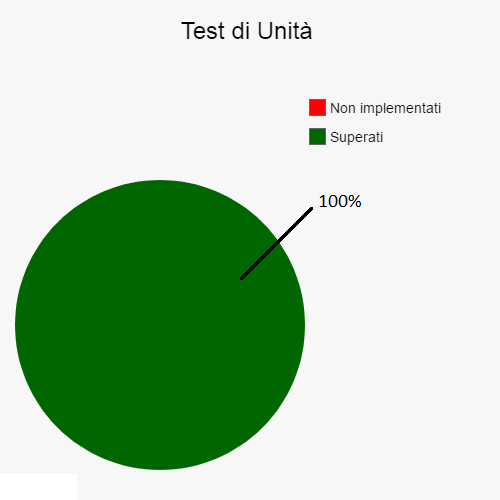
\includegraphics[scale=0.7]{includes/img/test_unita.png}
		\caption{Grado di completamento test di unità}
	\end{figure}
	
	\clearpage
	
	\subsection{Test di integrazione}
	Questa tipologia di test serve a verificare il corretto funzionamento delle singole componenti di sistema progettate durante l'attività di progettazione ad alto livello. Per questa tipologia di test, l'idea è quella di utilizzare un approccio top-down, in modo da sottoporre a test e integrare per primi i moduli di livello più alto.
	Così facendo, però, sarà necessario simulare le componenti di livello inferiore con degli stub. Una volta codificate, le componenti di livello più basso dovranno essere a loro volta integrate e testate.\\
	L'approccio top-down rientra tra le strategie di integrazione incrementale, che consentono di poter determinare in modo più rapido quale componente è la causa di problemi, poichè i difetti rilevati dai test saranno da attribuirsi all'ultima componente aggiunta.
	I test di integrazione saranno descritti nel modo seguente:
	\begin{center}
		\textbf{TI}[\textit{IdComponente}]
	\end{center}
	dove:
	\begin{itemize}
		\item
		\textbf{IdComponente} rappresenta il codice identificativo progressivo del componente preso in considerazione.
	\end{itemize}
	
	% TABELLA
	\normalsize
	\begin{longtable}{|>{\centering\arraybackslash}p{1.5cm}|>{\centering\arraybackslash}p{8cm} | >{\centering\arraybackslash}p{3.8cm}|}
		\hline \rowcolor{Gray}
		\textbf{Id Test} & \textbf{Descrizione} & \textbf{Stato}\\
		\hline
		\endhead
		\hypertarget{TI1}{TI1} & Viene verificato che l’applicazione web \progetto\ gestisca
		correttamente il front-end del prodotto e le sue interazioni con il back-end. & \textcolor{Green}{\textit{Superato}}\\ \hline
		\hypertarget{TI2}{TI2} & Viene verificato che i \textit{Controllers} del front-end si integrino
		correttamente nell’applicazione web. & \textcolor{Green}{\textit{Superato}}\\ \hline
		\hypertarget{TI3}{TI3} & Viene verificato che i \textit{Services} permettano una corretta interazione con il back-end. & \textcolor{Green}{\textit{Superato}}\\ \hline
		\hypertarget{TI4}{TI4} & Viene verificato che il \textit{Model} si integri correttamente con i
		\textit{Services} e con il resto delle componenti dell’applicazione che lo utilizzano. & \textcolor{Green}{\textit{Superato}}\\ \hline
		\hypertarget{TI5}{TI5} & Viene verificato che le \textit{Views} si integrino correttamente con i
		\textit{Controllers}, in modo da visualizzare senza errori i dati ricevuti. & \textcolor{Green}{\textit{Superato}}\\ \hline
		\hypertarget{TI6}{TI6} & Viene verificato che l’applicazione web gestisca	correttamente il back-end del prodotto, in modo tale da fornire al front-end le informazioni richieste. & \textcolor{Green}{\textit{Superato}}\\ \hline
		\hypertarget{TI7}{TI7} & Viene verificato che il \textit{Server} sia configurato e che sia in grado di caricare correttamente tutte le librerie necessarie all'istanziazione delle classi in modo corretto. & \textit{Non implementato}\\ \hline
		\hypertarget{TI8}{TI8} & Viene verificato che la \textit{Single Page App} si integri correttamente con i microservizi \textit{Jolie} utilizzati per il back-end. & \textcolor{Green}{\textit{Superato}}\\ \hline
		\hypertarget{TI9}{TI9} & Viene verificato che i \textit{Controllers} si integrino correttamente
		e gestiscano le richieste inoltrate dai \textit{Routers}. & \textcolor{Green}{\textit{Superato}}\\ \hline
		\hypertarget{TI10}{TI10} & Viene verificato che il \textit{Model} si integri correttamente con i
		\textit{Controllers} per la gestione dell’inserimento, della modifica e della cancellazione dei dati. & \textcolor{Green}{\textit{Superato}}\\ \hline
		\caption[Test di integrazione]{Test di integrazione}
		\label{tabella:test1}
	\end{longtable}

	\subsubsection{Grado di completamento dei test di integrazione}
	Di seguito viene fornito un pie chart che rappresenta il grado di completamento dei \textbf{test di integrazione} implementati e superati.
	\begin{figure}[H]
		\centering
		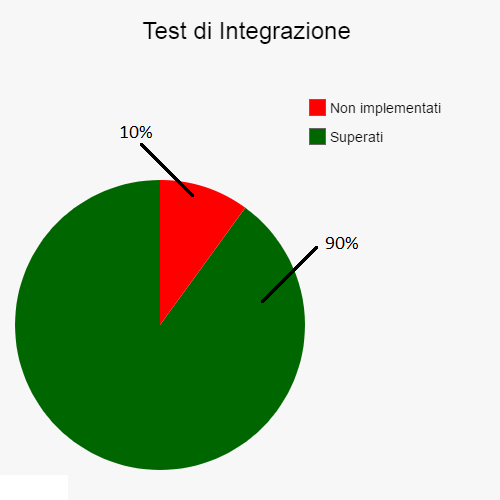
\includegraphics[scale=0.7]{includes/img/test_integrazione.png}
		\caption{Grado di completamento test di integrazione}
	\end{figure}

	\clearpage
	
	\subsection{Test di sistema}
	Questa tipologia di test serve a verificare il corretto comportamento e funzionamento dell’architettura. Tale tipologia di test deve verificare che ci sia la copertura totale dei requisiti software stabiliti durante l'\AdR.
	I test di sistema saranno organizzati nel modo seguente:
	\begin{center}
		\textbf{TS}[\textit{TipologiaRequisito}][\textit{RilevanzaRequisito}][\textit{CodiceRequisito}]
	\end{center}
	dove:
	\begin{itemize}
		\item
		\textbf{TipologiaRequisito} può assumere valori tra:
		\begin{itemize}
			\item
			\textit{V} per i requisiti di vincolo;
			\item
			\textit{F} per i requisiti di funzionalità;
			\item
			\textit{Q} per i requisiti di qualità;
			\item
			\textit{P} per i requisiti prestazionali.
		\end{itemize}
		\item 
		\textbf{RilevanzaRequisito} può assumere valori tra:
		\begin{itemize}
			\item
			\textit{O} per i requisiti obbligatori;
			\item
			\textit{D} per i requisiti desiderabili;
			\item
			\textit{F} per i requisiti facoltativi.
		\end{itemize}
		\item
		\textbf{CodiceRequisito} assume un valore gerarchico che identifica il singolo requisito.
	\end{itemize}
	
	% TABELLA
	\normalsize
	\begin{longtable}{|>{\centering\arraybackslash}p{2.3cm}|>{\centering\arraybackslash}p{7.5cm} | >{\centering\arraybackslash}p{3.8cm}|}
		\hline \rowcolor{Gray}
		\textbf{Id Test} & \textbf{Descrizione} & \textbf{Stato}\\
		\hline
		\endhead
		\hypertarget{TSFO1}{TSFO1} & Viene verificato che il sistema registri correttamente un utente. & \textcolor{Green}{\textit{Superato}}\\ \hline
		\hypertarget{TSFO2}{TSFO2} & Viene verificato che il sistema riesca a far effettuare correttamente il login ad un utente attraverso \progetto. & \textcolor{Green}{\textit{Superato}}\\ \hline	
		\hypertarget{TSFD3}{TSFD3} & Viene verificato che il sistema permetta il recupero della password per un utente registrato ad \progetto. & \textit{Non Implementato}\\ \hline	
		\hypertarget{TSFO4}{TSFO4} & Viene verificato che il sistema ricerchi correttamente una API. & \textcolor{Green}{\textit{Superato}}\\ \hline
		\hypertarget{TSFO4.3}{TSFO4.3} & Viene verificato che il sistema restituisca un insieme di risultati coerenti secondo i parametri di ricerca specificati da un utente. & \textcolor{Green}{\textit{Superato}}\\ \hline	
		\hypertarget{TSFO5}{TSFO5} & Viene verificato che il sistema visualizzi correttamente i dati relativi ad una API. & \textcolor{Green}{\textit{Superato}}\\ \hline
		\hypertarget{TSFO5.6}{TSFO5.6} & Viene verificato che il sistema consenta la consultazione della documentazione di una API. & \textcolor{Green}{\textit{Superato}}\\ \hline
		\hypertarget{TSFO5.7}{TSFO5.7} & Viene verificato che il sistema visualizzi correttamente i dati di utilizzo di una API. & \textit{Non Implementato}\\ \hline
		\hypertarget{TSFO6.2}{TSFO6.2} & Viene verificato che il sistema visualizzi correttamente la lista di API acquistate da un utente. & \textcolor{Green}{\textit{Superato}}\\ \hline
		\hypertarget{TSFO7}{TSFO7} & Viene verificato che il sistema consenta l'acquisto di una API, con conseguente rilascio di una API Key, per un utente. & \textcolor{Green}{\textit{Superato}}\\ \hline
		\hypertarget{TSFO7.5.3}{TSFO7.5.3} & Viene verificato che il sistema crei e visualizzi correttamente l'API Key associata ad una API, per cui è stata acquistata una licenza da un utente. & \textcolor{Green}{\textit{Superato}}\\ \hline
		\hypertarget{TSFO8}{TSFO8} & Viene verificato che il sistema gestisca correttamente le API inserite da uno sviluppatore. & \textcolor{Green}{\textit{Superato}}\\ \hline
		\hypertarget{TSFO8.2}{TSFO8.2} & Viene verificato che il sistema visualizzi correttamente la lista delle API registrate da uno sviluppatore. & \textcolor{Green}{\textit{Superato}}\\ \hline
		\hypertarget{TSFO8.2.4}{TSFO8.2.4} & Viene verificato che il sistema modifichi correttamente le informazioni relative ad una API registrata da uno sviluppatore. & \textcolor{Green}{\textit{Superato}}\\ \hline
		\hypertarget{TSFO8.2.8}{TSFO8.2.8} & Viene verificato che il sistema visualizzi correttamente il guadagno netto, in base alla policy, di una API da lui inserita. & \textit{Non Implementato}\\ \hline
		\hypertarget{TSFO8.2.9}{TSFO8.2.9} & Viene verificato che il sistema elimini correttamente una API su richiesta dello sviluppatore autore. & \textcolor{Green}{\textit{Superato}}\\ \hline
		\hypertarget{TSFO9}{TSFO9} & Viene verificato che il sistema inserisca correttamente nel marketplace una nuova API. & \textcolor{Green}{\textit{Superato}}\\ \hline
		\hypertarget{TSFO10.1}{TSFO10.1} & Viene verificato che il sistema permetta di gestire correttamente ad un utente le informazioni del proprio profilo. & \textcolor{Green}{\textit{Superato}}\\ \hline
		\hypertarget{TSFO10.1.1}{TSFO10.1.1} & Viene verificato che il sistema visualizzi correttamente le informazioni del profilo di un utente. & \textcolor{Green}{\textit{Superato}}\\ \hline
		\hypertarget{TSFO10.1.2}{TSFO10.1.2} & Viene verificato che il sistema modifichi correttamente le informazioni di un utente. & \textcolor{Green}{\textit{Superato}}\\ \hline
		\hypertarget{TSFD10.1.2.9}{TSFD10.1.2.9} & Viene verificato che il sistema effettui correttamente l'upgrade dell'account di un utente. & \textit{Non Implementato}\\ \hline
		\hypertarget{TSFO10.2}{TSFO10.2} & Viene verificato che il sistema permetta di gestire correttamente ad un utente il proprio conto. & \textcolor{Green}{\textit{Superato}}\\ \hline
		\hypertarget{TSFO10.2.1}{TSFO10.2.1} & Viene verificato che il sistema visualizzi correttamente il saldo attuale del conto di un utente. & \textcolor{Green}{\textit{Superato}}\\ \hline
		\hypertarget{TSFO10.2.2}{TSFO10.2.2} & Viene verificato che il sistema permetta ad un utente di ricaricare il saldo del proprio conto attraverso PayPal. & \textit{Non Implementato}\\ \hline
		\hypertarget{TSFO10.3}{TSFO10.3} & Viene verificato che il sistema visualizzi correttamente lo storico delle transazioni di un utente. & \textcolor{Green}{\textit{Superato}}\\ \hline
		\hypertarget{TSFO10.3.2}{TSFO10.3.2} & Viene verificato che il sistema visualizzi correttamente la lista delle transazioni concluse di un utente. & \textcolor{Green}{\textit{Superato}}\\ \hline
		\hypertarget{TSFO11}{TSFO11} & Viene verificato che il sistema riesca a far effettuare correttamente il logout ad un utente.  & \textcolor{Green}{\textit{Superato}}\\ \hline
		\hypertarget{TSFO12.1.1.1}{TSFO12.1.1.1} & Viene verificato che il sistema visualizzi correttamente i dati avanzati di una API da parte di un amministratore. & \textit{Non Implementato}\\ \hline
		\hypertarget{TSFO12.1.1.2}{TSFO12.1.1.2} & Viene verificato che il sistema sospenda correttamente una API su richiesta di un amministratore. & \textcolor{Green}{\textit{Superato}}\\ \hline
		\hypertarget{TSFD12.1.1.3}{TSFD12.1.1.3} & Viene verificato che il sistema elimini correttamente una API su richiesta di un amministratore. & \textcolor{Green}{\textit{Superato}}\\ \hline
		\hypertarget{TSFO12.2.1.1}{TSFO12.2.1.1} & Viene verificato che il sistema permetta ad un amministratore di sospendere correttamente un utente. & \textcolor{Green}{\textit{Superato}}\\ \hline
		\hypertarget{TSFO12.2.1.2}{TSFO12.2.1.2} & Viene verificato che il sistema permetta ad un amministratore di sospendere correttamente i pagamenti veso un utente. & \textit{Non Implementato}\\ \hline
		\hypertarget{TSFO12.2.1.3}{TSFO12.2.1.3} & Viene verificato che il sistema permetta ad un amministratore di revocare correttamente la sospensione ad un utente sospeso. & \textcolor{Green}{\textit{Superato}}\\ \hline
		\hypertarget{TSFO12.2.1.5}{TSFO12.2.1.5} & Viene verificato che il sistema permetta ad un amministratore di eliminare correttamente un utente. & \textcolor{Green}{\textit{Superato}}\\ \hline		
		\hypertarget{TSVO1}{TSVO1} & Viene verificato che il sistema abbia un'architettura a microservizi. & \textcolor{Green}{\textit{Superato}}\\ \hline
		\hypertarget{TSVO2}{TSVO2} & Viene verificato che il sistema utilizzi il linguaggio \textit{Jolie} per l'API Gateway, il back-end dell'applicazione web e le interfacce dei microservizi. & \textcolor{Green}{\textit{Superato}}\\ \hline
		\hypertarget{TSVO3}{TSVO3} & Viene verificato che il sistema utilizzi il linguaggio di markup \textit{HTML5}, unito a fogli di stile in \textit{CSS3} e linguaggio di scripting \textit{JavaScript}. & \textcolor{Green}{\textit{Superato}}\\ \hline
		\hypertarget{TSVO4}{TSVO4} & Viene verificato che il sistema utilizzi il DBMS di tipo relazionale \textit{MySQL}. & \textcolor{Green}{\textit{Superato}}\\ \hline
		\hypertarget{TSVO5}{TSVO5} & Viene verificato che il sistema funzioni su \textit{Google Chrome} versione 55.0 o superiore & \textcolor{Green}{\textit{Superato}}\\ \hline
		\hypertarget{TSVO6}{TSVO6} & Viene verificato che il sistema funzioni su \textit{Mozilla Firefox} versione 51.0 o superiore & \textcolor{Green}{\textit{Superato}}\\ \hline
		\hypertarget{TSVO7}{TSVO7} & Viene verificato che il sistema funzioni su \textit{Safari} versione 10.0 o superiore & \textcolor{Green}{\textit{Superato}}\\ \hline
		\hypertarget{TSVD8}{TSVD8} & Viene verificato che il sistema funzioni su \textit{Opera} versione 42.0 o superiore & \textcolor{Green}{\textit{Superato}}\\ \hline
		\hypertarget{TSVD9}{TSVD9} & Viene verificato che il sistema funzioni su \textit{Internet Explorer} versione 11.0 o superiore & \textcolor{Green}{\textit{Superato}}\\ \hline
		\hypertarget{TSVO10}{TSVO10} & Viene verificato che il sistema funzioni su \textit{Microsoft Edge} versione 38.0 o superiore & \textcolor{Green}{\textit{Superato}}\\ \hline
		\hypertarget{TSVO11}{TSVO11} & Viene verificato che il sistema funzioni su \textit{Android Browser} versione 5.1 o superiore & \textcolor{Green}{\textit{Superato}}\\ \hline
		\hypertarget{TSVO12}{TSVO12} & Viene verificato che il sistema funzioni su \textit{Safari} per iOS 10 o versioni superiori & \textcolor{Green}{\textit{Superato}}\\ \hline
		\hypertarget{TSVF13}{TSVF13} & Viene verificato che il sistema funzioni su \textit{Google Chrome} per iOS versione 56.0 o superiore & \textit{Non Implementato}\\ \hline
		\hypertarget{TSVD14}{TSVD14} & Viene verificato che il sistema funzioni su \textit{Google Chrome} per Android versione 56.0 o superiore & \textit{Non Implementato}\\ \hline
		\caption[Test di sistema]{Test di sistema}
		\label{tabella:test2}
	\end{longtable}
	
	\subsubsection{Grado di completamento dei test di sistema}
	Di seguito viene fornito un pie chart che rappresenta il grado di completamento dei \textbf{test di sistema} implementati e superati.
	\begin{figure}[H]
		\centering
		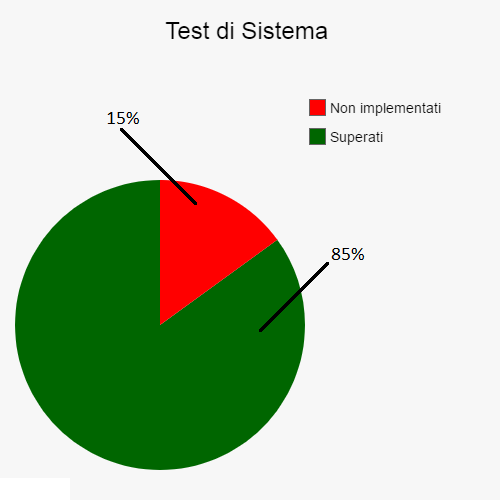
\includegraphics[scale=0.7]{includes/img/test_sistema.png}
		\caption{Grado di completamento test di sistema}
	\end{figure}	
	
	\clearpage
	
	\subsection{Test di non regressione}
	Questa tipologia di test consiste nell'eseguire nuovamente i test che coinvolgono le componenti software che hanno subito modifiche, in modo da verificare che i cambiamenti apportati non compromettano il funzionamento di componenti che non sono stati aggiornati e che, precedentemente, non erano soggetti ad errori.\\
	I test di non regressione saranno descritti nel modo seguente:
	\begin{center}
		\textbf{TNR}[\textit{IdTest}]
	\end{center}
	dove \textbf{\textit{IdTest}} rappresenta il codice identificativo progressivo della modifica apportata, la quale ha prodotto il corrispondente test di non regressione.
	
	% TABELLA
	\normalsize
	\begin{longtable}{|>{\centering\arraybackslash}p{1.5cm}|>{\centering\arraybackslash}p{8cm} | >{\centering\arraybackslash}p{3.8cm}|}
		\hline \rowcolor{Gray}
		\textbf{Id Test} & \textbf{Descrizione} & \textbf{Stato}\\
		\hline
		\endhead
		\hypertarget{TNR1}{TNR1} & Descrizione... & \textcolor{Green}{\textit{Superato}}\\ \hline
		\hypertarget{TNR2}{TNR2} & Descrizione... & \textcolor{Green}{\textit{Superato}}\\ \hline
		\hypertarget{TNR3}{TNR3} & Descrizione... & \textcolor{Green}{\textit{Superato}}\\ \hline
		\hypertarget{TNR4}{TNR4} & Descrizione... & \textcolor{Green}{\textit{Superato}}\\ \hline
		\caption[Test di non regressione]{Test di non regressione}
		\label{tabella:test3}
	\end{longtable}
	
	\subsubsection{Grado di completamento dei test di non regressione}
	Di seguito viene fornito un pie chart che rappresenta il grado di completamento dei \textbf{test di non regressione} implementati e superati.
	\begin{figure}[H]
		\centering
		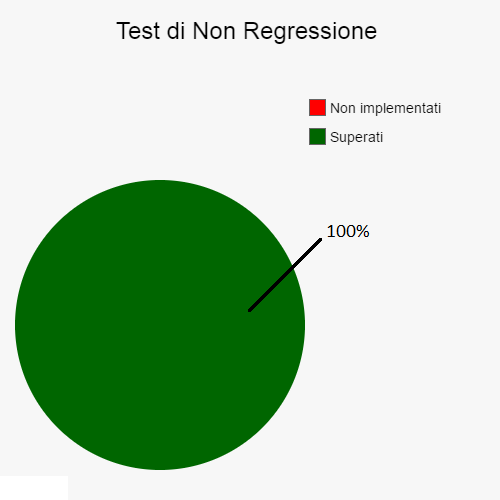
\includegraphics[scale=0.7]{includes/img/test_non_regressione.png}
		\caption{Grado di completamento test di non regressione}
	\end{figure}	
	
	\clearpage
	
	\subsection{Test di validazione}
	Questa tipologia di test serve a verificare che il prodotto soddisfi le richieste del proponente attraverso le funzionalità implementate.\\
	Per questo motivo, occorrerà simulare il comportamento generale dell'applicativo e dell'utente che interagisce con esso, attraverso delle macro azioni.\\
	I test di validazione saranno organizzati nel modo seguente:
	\begin{center}
		\textbf{TV}[\textit{TipologiaRequisito}][\textit{RilevanzaRequisito}][\textit{CodiceRequisito}]
	\end{center}
	dove:
	\begin{itemize}
		\item
		\textbf{TipologiaRequisito} può assumere valori tra:
		\begin{itemize}
			\item
			\textit{V} per i requisiti di vincolo;
			\item
			\textit{F} per i requisiti di funzionalità;
			\item
			\textit{Q} per i requisiti di qualità;
			\item
			\textit{P} per i requisiti prestazionali.
		\end{itemize}
		\item 
		\textbf{RilevanzaRequisito} può assumere valori tra:
		\begin{itemize}
			\item
			\textit{O} per i requisiti obbligatori;
			\item
			\textit{D} per i requisiti desiderabili;
			\item
			\textit{F} per i requisiti facoltativi.
		\end{itemize}
		\item
		\textbf{CodiceRequisito} assume un valore gerarchico che identifica il singolo requisito.
	\end{itemize}

	% TABELLA
	\normalsize
	\begin{longtable}{|>{\centering\arraybackslash}p{2.3cm}|>{\centering\arraybackslash}p{7.5cm} | >{\centering\arraybackslash}p{4cm}|}
		\hline \rowcolor{Gray}
		\textbf{Id Test} & \textbf{Descrizione} & \textbf{Stato}\\
		\hline
		\endhead
		\hypertarget{TVFO1}{TVFO1} & L’utente intende registrarsi alla piattaforma \progetto. All’utente è richiesto di:
		\begin{itemize}
			\item Trovarsi nella sezione apposita;
			\item Compilare il form di registrazione;
			\item Premere il pulsante di conferma;
			\item Verificare attraverso l’autenticazione che la registrazione sia avvenuta correttamente.
		\end{itemize}
		& \textcolor{Green}{\textit{Superato}}\\ \hline
		\hypertarget{TVFO2}{TVFO2} & L’utente intende autenticarsi alla piattaforma \progetto. All’utente è richiesto di:
		\begin{itemize}
			\item Trovarsi nella sezione apposita;
			\item Essere in possesso delle credenziali richieste;
			\item Inserire le credenziali nell’apposito form;
			\item Premere il pulsante di autenticazione;
			\item Verificare che l’autenticazione sia effettivamente avvenuta.
		\end{itemize}
		& \textcolor{Green}{\textit{Superato}}\\ \hline
		\hypertarget{TVFO4}{TVFO4} & L’utente autenticato  intende ricercare una API sul marketplace. All’utente è richiesto di:
		\begin{itemize}
			\item Trovarsi nella sezione apposita;
			\item Ricercare una API digitando le keywords;
			\item Visualizzazione dei risultati della ricerca, secondo le keywords specificate.
		\end{itemize} & \textcolor{Green}{\textit{Superato}}\\ \hline
		\hypertarget{TVFO5}{TVFO5} & L’utente autenticato  intende visualizzare le informazioni relative ad una API. All’utente è richiesto di:
		\begin{itemize}
			\item Trovarsi nella sezione apposita;
			\item Selezionare l'API di cui vuole visualizzare le informazioni;
			\item Visualizzazione dei dati relativi alla API selezionata.
		\end{itemize} & \textcolor{Green}{\textit{Superato}}\\ \hline
		\hypertarget{TVFO5.6}{TVFO5.6} & L’utente autenticato  intende consultare la documentazione relativa ad una API. All’utente è richiesto di:
		\begin{itemize}
			\item Trovarsi nella sezione apposita;
			\item Selezionare l'API di interesse;
			\item Visualizzazione della documentazione dell'API.
		\end{itemize} & \textcolor{Green}{\textit{Superato}}\\ \hline
		\hypertarget{TVFO7}{TVFO7} & L’utente autenticato intende acquistare l'API che sta visualizzando. All’utente è richiesto di:
		\begin{itemize}
			\item Essere autenticato;
			\item Trovarsi nella sezione apposita;
			\item Selezionare la policy di vendita;
			\item Confermare l'acquisto attraverso l'apposito pulsante;
			\item Verificare la transazione nel proprio storico.
		\end{itemize} & \textcolor{Green}{\textit{Superato}}\\ \hline
		\hypertarget{TVFO8.2}{TVFO8.2} & L’utente sviluppatore intende visualizzare l'elenco di API da lui caricate sulla piattaforma \progetto. All’utente è richiesto di:
		\begin{itemize}
			\item Essere autenticato;
			\item Trovarsi nella sezione apposita;
			\item Verificare che vengano visualizzati tutte le proprie API inserite.
		\end{itemize} & \textcolor{Green}{\textit{Superato}}\\ \hline
		\hypertarget{TVFO8.2.3}{TVFO8.2.3} & L’utente sviluppatore intende visualizzare il numero di licenze attive per le API da lui caricate sulla piattaforma \progetto. All’utente è richiesto di:
		\begin{itemize}
			\item Essere autenticato;
			\item Trovarsi nella sezione apposita;
			\item Selezionare una API dall'elenco visualizzato;
			\item Verificare che vengao il numero di licenze attive per la propria API registrata.
		\end{itemize} & \textcolor{Green}{\textit{Superato}}\\ \hline
		\hypertarget{TVFO8.2.4}{TVFO8.2.4} & L’utente sviluppatore intende modificare i dati relativi ad una sua API caricata. All’utente è richiesto di:
		\begin{itemize}
			\item Essere autenticato;
			\item Trovarsi nella sezione apposita;
			\item Premere il pulsante "Modifica API";
			\item Modificare i dati dell'API selezionata;
			\item Premere il pulsante di conferma modifica;
			\item Verificare che sia stata modificata l'API.
		\end{itemize} & \textcolor{Green}{\textit{Superato}}\\ \hline
		\hypertarget{TVFO9}{TVFO9} & L’utente sviluppatore intende caricare una propria API sulla piattaforma \progetto. All’utente è richiesto di:
		\begin{itemize}
			\item Essere autenticato;
			\item Trovarsi nella sezione apposita;
			\item Premere il pulsante "Inserisci API";
			\item Inserire i dati necessari alla pubblicazione della propria API;
			\item Premere il pulsante di conferma inserimento nuova API;
			\item Verificare che sia stata aggiunta al marketplace l'API.
		\end{itemize} & \textcolor{Green}{\textit{Superato}}\\ \hline
		\hypertarget{TVFO10.1.1}{TVFO10.1.1} & L’utente autenticato intende visualizzare il proprio profilo. All’utente è richiesto di:
		\begin{itemize}
			\item Essere autenticato;
			\item Trovarsi nella sezione apposita;
			\item Visualizzare il proprio profilo.
		\end{itemize} & \textcolor{Green}{\textit{Superato}}\\ \hline
		\hypertarget{TVFO10.1.2}{TVFO10.1.2} & L’utente autenticato intende modificare i propri dati. All’utente è richiesto di:
		\begin{itemize}
			\item Essere autenticato;
			\item Trovarsi nella sezione apposita;
			\item Modificare i campi dati consentiti;
			\item Premere il tasto "Conferma Modifiche";
			\item Visualizzare il profilo dell’utente modificato.
		\end{itemize}
		& \textcolor{Green}{\textit{Superato}}\\ \hline
		\hypertarget{TVFD10.1.2.9}{TVFD10.1.2.9} & L’utente autenticato  intende modificare la tipologia di utenza, effettuando un upgrade dell'account. All’utente è richiesto di:
		\begin{itemize}
			\item Essere autenticato;
			\item Trovarsi nella sezione apposita;
			\item Effettuare l'upgrade dell'account, passando da "cliente" a "sviluppatore";
			\item Verificare la modifica effettuata.
		\end{itemize} & \textcolor{Green}{\textit{Superato}}\\ \hline
		\hypertarget{TVFO10.2.1}{TVFO10.2.1} & L’utente intende visualizzare il saldo del proprio conto associato all'account. All’utente è richiesto di:
		\begin{itemize}
			\item Essere autenticato;
			\item Trovarsi nella sezione apposita;
			\item Premere il pulsante "Conto Virtuale";
			\item Visualizzazione del saldo attuale del proprio conto.
		\end{itemize} & \textcolor{Green}{\textit{Superato}}\\ \hline
		\hypertarget{TVFO10.3}{TVFO10.3} & L’utente autenticato intende visualizzare lo storico delle transazioni effettuate. All’utente è richiesto di:
		\begin{itemize}
			\item Essere autenticato;
			\item Trovarsi nella sezione apposita;
			\item Visualizzare lo storico delle transazioni.
		\end{itemize} & \textcolor{Green}{\textit{Superato}}\\ \hline		
		\hypertarget{TVFO11}{TVFO11} & L’utente intende disconnettersi dalla piattaforma \progetto. All’utente è richiesto di:
		\begin{itemize}
			\item Essere autenticato;
			\item Trovarsi nella sezione apposita;
			\item Premere il pulsante di logout;
			\item Verificare che la disconnessione sia effettivamente avvenuta.
		\end{itemize}
		& \textcolor{Green}{\textit{Superato}}\\ \hline
		\hypertarget{TVFO12.2.1}{TVFO12.2.1} & L’utente amministratore della piattaforma \progetto\ intende moderare un determinato utente registrato. All’utente è richiesto di:
		\begin{itemize}
			\item Essere autenticato;
			\item Trovarsi nella sezione apposita;
			\item Selezionare l'utente che si vuole moderare;
			\item Inserire i dati del rapporto di moderazione;
			\item Verificare che l'utente sia stato effettivamente moderato.
		\end{itemize} & \textcolor{Green}{\textit{Superato}}\\ \hline
		\caption[Test di validazione]{Test di validazione}
		\label{tabella:test4}
	\end{longtable}

	\subsubsection{Grado di completamento dei test di validazione}
	Di seguito viene fornito un pie chart che rappresenta il grado di completamento dei \textbf{test di validazione} implementati e superati.
	\begin{figure}[H]
		\centering
		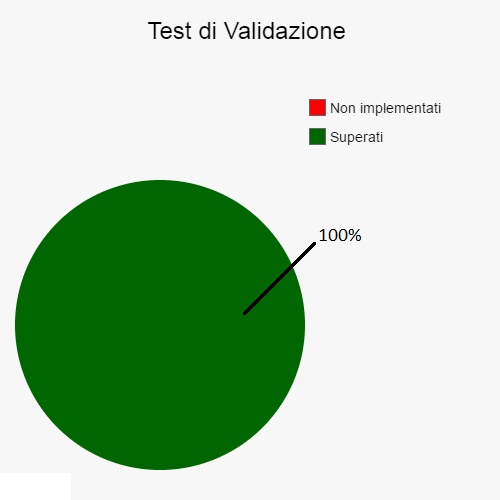
\includegraphics[scale=0.7]{includes/img/test_validazione.png}
		\caption{Grado di completamento test di validazione}
	\end{figure}
	
	\clearpage
\appendix
\newpage
\section{Resoconto verifica documenti}

In questa sezione del documento vengono descritti e analizzati gli esiti delle attività di verifica svolte su tutti i documenti che vengono consegnati nelle varie revisioni di avanzamento del progetto.
L’analisi dei documenti mediante la tecnica \textit{Walkthrough} ha reso possibile individuare alcuni errori frequenti, che si sono aggiunti alla lista di controllo stilata ed aggiornata nelle varie revisioni, utile per applicare la tecnica \textit{Inspection} nelle future attività di verifica.\\
Il team, attraverso il software interno \textit{NetBreakDB}, è riuscito ad effettuare i tracciamenti per le componenti di interesse previste da ogni revisione (casi d’uso-requisiti, requisiti-fonti, requisiti-componenti, requisiti-classi, etc.).\\
Inoltre, questo software è stato utilizzato per generare le tabelle dei vari test e dei relativi tracciamenti con requisiti, componenti, classi e metodi.
	
	\subsection{Revisione dei Requisiti}
	Di seguito, sono riportati gli esiti delle verifiche sottoposte a tutti i documenti, per il calcolo della metrica \textit{Indice Gulpease} (\hyperlink{MPC19}{MPC19}).
	
		\begin{longtable}{|>{\centering\arraybackslash}p{5.5cm}|>{\centering\arraybackslash}p{5cm} | >{\centering\arraybackslash}p{5cm}|}
			\hline
			\rowcolor{Gray}
			\textbf{Documento} & \textbf{Indice Gulpease} & \textbf{Esito} \\
			\hline
			\textit{\NdP\ 1.0.0} & 49 & \textcolor{Green}{\textit{Superato}}\\
			\hline
			\textit{\PdP\ 1.0.0} & 50 & \textcolor{Green}{\textit{Superato}} \\
			\hline
			\textit{\PdQ\ 1.0.0} & 42 & \textcolor{Green}{\textit{Superato}}\\
			\hline
			\textit{\AdR\ 1.0.0} & 68 & \textcolor{Green}{\textit{Superato}} \\
			\hline
			\textit{\SdF\ 1.0.0} & 54 & \textcolor{Green}{\textit{Superato}}\\
			\hline
			\textit{\G\ 1.0.0}& 43 & \textcolor{Green}{\textit{Superato}}\\
			\hline
			\textit{Verbale Interno - 28/11/2016}		& 	60	&	\textcolor{Green}{\textit{Superato}}	\\
			\hline
			\textit{Verbale Interno - 01/12/2016}		& 	63	&	\textcolor{Green}{\textit{Superato}}	\\
			\hline
			\textit{Verbale Interno - 12/12/2016}		& 	61	&	\textcolor{Green}{\textit{Superato}}	\\
			\hline
			\textit{Verbale Esterno - 22/12/2016}		& 	59	&	\textcolor{Green}{\textit{Superato}}	\\
			\hline
			\textit{Verbale Interno - 28/12/2016}		& 	61	&	\textcolor{Green}{\textit{Superato}}	\\
			\hline
		
		\caption{Resoconto verifiche documenti - RR}
	\end{longtable}

\newpage	
	\subsection{Revisione di Progettazione}
	Di seguito, sono riportati gli esiti delle verifiche sottoposte a tutti i documenti, per il calcolo della metrica \textit{Indice Gulpease} (\hyperlink{MPC19}{MPC19}).
	
			\begin{longtable}{|>{\centering\arraybackslash}p{5.5cm}|>{\centering\arraybackslash}p{5cm} | >{\centering\arraybackslash}p{5cm}|}
				\hline
				\rowcolor{Gray}
				\textbf{Documento} & \textbf{Indice Gulpease} & \textbf{Esito} \\
				\hline
				\textit{\ST\ 1.0.0} & 67  & \textcolor{Green}{\textit{Superato}}\\
				\hline
				\textit{\NdP\ 2.0.0} & 57  & \textcolor{Green}{\textit{Superato}}\\
				\hline
				\textit{\PdP\ 2.0.0} & 55 & \textcolor{Green}{\textit{Superato}} \\
				\hline
				\textit{\PdQ\ 2.0.0} & 54  & \textcolor{Green}{\textit{Superato}}\\
				\hline
				\textit{\AdR\ 2.0.0} & 70  & \textcolor{Green}{\textit{Superato}} \\
				\hline
				\textit{\G\ 2.0.0}& 49 & \textcolor{Green}{\textit{Superato}}\\
				\hline
				\textit{Verbale Interno - 27/01/2017}		& 	55	&	\textcolor{Green}{\textit{Superato}}	\\
				\hline
				\textit{Verbale Interno - 04/02/2017}		& 	64	&	\textcolor{Green}{\textit{Superato}}	\\
				\hline
				\textit{Verbale Interno - 13/02/2017}		& 	58	&	\textcolor{Green}{\textit{Superato}}	\\
				\hline
				\textit{Verbale Esterno - 16/02/2017}		& 	60	&	\textcolor{Green}{\textit{Superato}}	\\
				\hline
				\textit{Verbale Interno - 17/02/2017}		& 	57	&	\textcolor{Green}{\textit{Superato}}	\\
				\hline
				\textit{Verbale Interno - 21/02/2017}		& 	63	&	\textcolor{Green}{\textit{Superato}}	\\
				\hline
				\textit{Verbale Interno - 02/03/2017}		& 	61	&	\textcolor{Green}{\textit{Superato}}	\\
				\hline
				\textit{Verbale Interno - 03/03/2017}		& 	61	&	\textcolor{Green}{\textit{Superato}}	\\
				\hline
			
			\caption{Resoconto verifiche documenti - RP}
		\end{longtable}

\newpage
	\subsection{Revisione di Qualifica}
	Di seguito, sono riportati gli esiti delle verifiche sottoposte a tutti i documenti, per il calcolo della metrica \textit{Indice Gulpease} (\hyperlink{MPC19}{MPC19}).
	
			\begin{longtable}{|>{\centering\arraybackslash}p{5.7cm}|>{\centering\arraybackslash}p{5cm} | >{\centering\arraybackslash}p{5cm}|}
				\hline
				\rowcolor{Gray}
				\textbf{Documento} & \textbf{Indice Gulpease} & \textbf{Esito} \\
				\hline
				\textit{\DDP\ 1.0.0} & 72 & \textcolor{Green}{\textit{Superato}}\\
				\hline
				\textit{\MU\ 1.0.0} & 68 & \textcolor{Green}{\textit{Superato}}\\
				\hline
				\textit{\ST\ 2.0.0} & 69  & \textcolor{Green}{\textit{Superato}}\\
				\hline
				\textit{\NdP\ 3.0.0} & 61  & \textcolor{Green}{\textit{Superato}}\\
				\hline
				\textit{\PdP\ 3.0.0} & 60 & \textcolor{Green}{\textit{Superato}} \\
				\hline
				\textit{\PdQ\ 3.0.0} &  63 & \textcolor{Green}{\textit{Superato}}\\
				\hline
				\textit{\AdR\ 3.0.0} &  71 & \textcolor{Green}{\textit{Superato}} \\
				\hline
				\textit{\G\ 3.0.0}& 50 & \textcolor{Green}{\textit{Superato}}\\
				\hline
				\textit{Tracciamento Verbali Interni RQ}		& 	68	&	\textcolor{Green}{\textit{Superato}}	\\
				\hline
				\textit{Tracciamento Verbali Esterni RQ}		& 	67	&	\textcolor{Green}{\textit{Superato}}	\\
				\hline
				\textit{Verbale Interno 2017-03-16}		& 	57	&	\textcolor{Green}{\textit{Superato}}	\\
				\hline
				\textit{Verbale Interno 2017-03-31}		& 	61	&	\textcolor{Green}{\textit{Superato}}	\\
				\hline
				\textit{Verbale Interno 2017-04-28}		& 	59	&	\textcolor{Green}{\textit{Superato}}	\\
				\hline
				\textit{Verbale Esterno 2017-03-17}		& 	60	&	\textcolor{Green}{\textit{Superato}}	\\
				\hline
				\textit{Verbale Esterno 2017-03-30}		& 	65	&	\textcolor{Green}{\textit{Superato}}	\\
				\hline
				\textit{Verbale Esterno 2017-04-06}		& 	62	&	\textcolor{Green}{\textit{Superato}}	\\
				\hline
				\textit{Verbale Esterno 2017-04-10}		& 	64	&	\textcolor{Green}{\textit{Superato}}	\\
				\hline
				\textit{Verbale Esterno 2017-04-13}		& 	61	&	\textcolor{Green}{\textit{Superato}}	\\
				\hline
				\textit{Verbale Esterno 2017-04-19}		& 	65	&	\textcolor{Green}{\textit{Superato}}	\\
				\hline
				\textit{Verbale Esterno 2017-04-24}		& 	59	&	\textcolor{Green}{\textit{Superato}}	\\
				\hline

			\caption{Resoconto verifiche documenti - RQ}
		\end{longtable}

\newpage
\subsection{Revisione di Accettazione}
Di seguito, sono riportati gli esiti delle verifiche sottoposte a tutti i documenti, per il calcolo della metrica \textit{Indice Gulpease} (\hyperlink{MPC19}{MPC19}).

\begin{longtable}{|>{\centering\arraybackslash}p{5.7cm}|>{\centering\arraybackslash}p{5cm} | >{\centering\arraybackslash}p{5cm}|}
	\hline
	\rowcolor{Gray}
	\textbf{Documento} & \textbf{Indice Gulpease} & \textbf{Esito} \\
	\hline
	\textit{\DDP\ 2.0.0} & xx & \textcolor{Green}{\textit{Superato}}\\
	\hline
	\textit{\MU\ 2.0.0} & xx & \textcolor{Green}{\textit{Superato}}\\
	\hline
	\textit{\MS\ 1.0.0} & xx & \textcolor{Green}{\textit{Superato}}\\
	\hline
	\textit{\ST\ 3.0.0} & xx  & \textcolor{Green}{\textit{Superato}}\\
	\hline
	\textit{\NdP\ 4.0.0} & 65  & \textcolor{Green}{\textit{Superato}}\\
	\hline
	\textit{\PdP\ 4.0.0} & xx & \textcolor{Green}{\textit{Superato}} \\
	\hline
	\textit{\PdQ\ 4.0.0} &  xx & \textcolor{Green}{\textit{Superato}}\\
	\hline
	\textit{\AdR\ 3.0.0} &  xx & \textcolor{Green}{\textit{Superato}} \\
	\hline
	\textit{\G\ 3.0.0}& xx & \textcolor{Green}{\textit{Superato}}\\
	\hline
	\textit{Verbale Interno 2017-xx-yy}		& 	xx	&	\textcolor{Green}{\textit{Superato}}	\\
	\hline
	\textit{Verbale Esterno 2017-xx-yy}		& 	xx	&	\textcolor{Green}{\textit{Superato}}	\\
	\hline
	
	\caption{Resoconto verifiche documenti - RA}
\end{longtable}

\subsection{Riepilogo}
Infine, per ogni documento principale, viene riportato un grafico che mostra la progressione e il rispettivo miglioramento del documento secondo l'\textit{indice Gulpease}.

\begin{figure}[H]
	\centering
	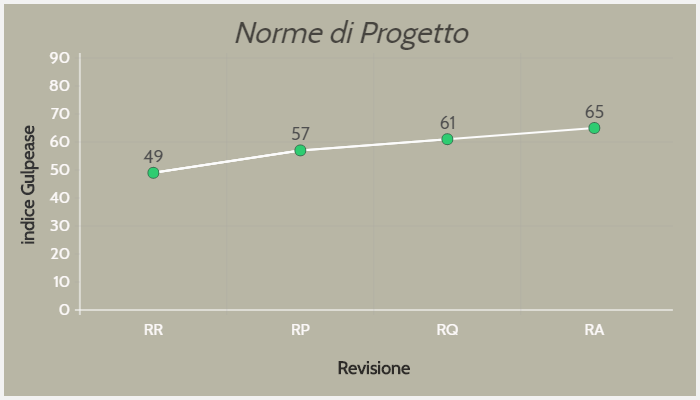
\includegraphics[scale=0.6]{includes/img/NdP.png}
	\caption{Miglioramento Norme di Progetto}
\end{figure}


\newpage
\section{Resoconto Qualità di Prodotto}

In questa sezione del documento vengono descritti e analizzati gli esiti delle metriche previste per il controllo della qualità di prodotto, in base alla revisione di progetto.

	\subsection{Revisione di Qualifica}
	
		\begin{longtable}{|>{\centering\arraybackslash}p{2cm}|>{\centering\arraybackslash}p{5cm}|>{\centering\arraybackslash}p{3cm}|>{\centering\arraybackslash}p{3cm}|}
			\hline
			\rowcolor{Gray}
			\textbf{Id} & \textbf{Metrica} & \textbf{Valore} & \textbf{Esito} \\
			\hline
				\hyperlink{MPDF1}{MPD\_F1} & \textit{Completezza delle funzioni sviluppate} & 93\% & \textcolor{Green}{\textit{Superato}}\\
				\hline
				\hyperlink{MPDF2}{MPD\_F2} & \textit{Correttezza delle funzioni sviluppate} & 100\% & \textcolor{Green}{\textit{Superato}}\\
				\hline
				\hyperlink{MPDF3}{MPD\_F3} & \textit{Accuratezza rispetto alle aspettative} & 91\% & \textcolor{Green}{\textit{Superato}}\\
				\hline
				\hyperlink{MPDF4}{MPD\_F4} & \textit{Controllo degli accessi} & 91\% & \textcolor{Green}{\textit{Superato}}\\
				\hline
				\hyperlink{MPDA1}{MPD\_A1} & \textit{Chiamate a microservizi corrette} & 96\% & \textcolor{Green}{\textit{Superato}}\\
				\hline
				\hyperlink{MPDA2}{MPD\_A2} & \textit{Copertura dei test} & 83\% & \textcolor{Green}{\textit{Superato}}\\
				\hline
				\hyperlink{MPDA3}{MPD\_A3} & \textit{Controllo dei guasti} & 84\% & \textcolor{Green}{\textit{Superato}}\\
				\hline
				\hyperlink{MPDU1}{MPD\_U1} & \textit{Comprensibilità delle funzionalità offerte} & 85\% & \textcolor{Green}{\textit{Superato}}\\
				\hline
				\hyperlink{MPDU2}{MPD\_U2} & \textit{Controllo e monitoraggio delle operazioni} & 89\% & \textcolor{Green}{\textit{Superato}}\\
				\hline
				\hyperlink{MPDU3}{MPD\_U3} & \textit{Qualità della messaggistica} & 81\% & \textcolor{Green}{\textit{Superato}}\\
				\hline
				\hyperlink{MPDE1}{MPD\_E1} & \textit{Tempo di risposta} & 4 & \textcolor{Green}{\textit{Superato}}\\
				\hline
				\hyperlink{MPDM1}{MPD\_M1} & \textit{Impatto delle modifiche} & 20\% & \textcolor{Green}{\textit{Superato}}\\
				\hline
				\hyperlink{MPDP1}{MPD\_P1} & \textit{Supporto differenti versioni dei browser} & 90\% & \textcolor{Green}{\textit{Superato}}\\
				\hline
			
			\caption{Resoconto esiti metriche - Qualità di prodotto RQ}
		\end{longtable}

	\subsection{Revisione di Accettazione}
	
	\begin{longtable}{|>{\centering\arraybackslash}p{2cm}|>{\centering\arraybackslash}p{5cm}|>{\centering\arraybackslash}p{3cm}|>{\centering\arraybackslash}p{3cm}|}
		\hline
		\rowcolor{Gray}
		\textbf{Id} & \textbf{Metrica} & \textbf{Valore} & \textbf{Esito} \\
		\hline
		\hyperlink{MPDF1}{MPD\_F1} & \textit{Completezza delle funzioni sviluppate} & xx\% & \textcolor{Green}{\textit{Superato}}\\
		\hline
		\hyperlink{MPDF2}{MPD\_F2} & \textit{Correttezza delle funzioni sviluppate} & xx\% & \textcolor{Green}{\textit{Superato}}\\
		\hline
		\hyperlink{MPDF3}{MPD\_F3} & \textit{Accuratezza rispetto alle aspettative} & xx\% & \textcolor{Green}{\textit{Superato}}\\
		\hline
		\hyperlink{MPDF4}{MPD\_F4} & \textit{Controllo degli accessi} & xx\% & \textcolor{Green}{\textit{Superato}}\\
		\hline
		\hyperlink{MPDA1}{MPD\_A1} & \textit{Chiamate a microservizi corrette} & xx\% & \textcolor{Green}{\textit{Superato}}\\
		\hline
		\hyperlink{MPDA2}{MPD\_A2} & \textit{Copertura dei test} & xx\% & \textcolor{Green}{\textit{Superato}}\\
		\hline
		\hyperlink{MPDA3}{MPD\_A3} & \textit{Controllo dei guasti} & xx\% & \textcolor{Green}{\textit{Superato}}\\
		\hline
		\hyperlink{MPDU1}{MPD\_U1} & \textit{Comprensibilità delle funzionalità offerte} & xx\% & \textcolor{Green}{\textit{Superato}}\\
		\hline
		\hyperlink{MPDU2}{MPD\_U2} & \textit{Controllo e monitoraggio delle operazioni} & xx\% & \textcolor{Green}{\textit{Superato}}\\
		\hline
		\hyperlink{MPDU3}{MPD\_U3} & \textit{Qualità della messaggistica} & xx\% & \textcolor{Green}{\textit{Superato}}\\
		\hline
		\hyperlink{MPDE1}{MPD\_E1} & \textit{Tempo di risposta} & xx & \textcolor{Green}{\textit{Superato}}\\
		\hline
		\hyperlink{MPDM1}{MPD\_M1} & \textit{Impatto delle modifiche} & xx\% & \textcolor{Green}{\textit{Superato}}\\
		\hline
		\hyperlink{MPDP1}{MPD\_P1} & \textit{Supporto differenti versioni dei browser} & xx\% & \textcolor{Green}{\textit{Superato}}\\
		\hline
		
		\caption{Resoconto esiti metriche - Qualità di prodotto RA}
	\end{longtable}
\newpage
\section{Resoconto Qualità di Processo}

In questa sezione del documento vengono descritti e analizzati gli esiti delle metriche previste per il controllo della qualità di processo, in base alla revisione di progetto.\\
La prima tabella contiene le metriche con associato esito applicate sull'intero sistema, mentre le successive tabelle sono una per ogni metrica che si applica a singole componenti.\\
\textbf{N.B.:} per una consultazione più semplice e rapida, per le metriche \textit{Numero di metodi per classe}, \textit{Numero di parametri per metodo} e \textit{Numero di attributi per classe} viene riportata una semplice tabella indicante il valore minimo, massimo e medio individuati tra tutte le classe o metodi implementate/i.\\
Nel caso in cui il valore massimo e/o minimo non rientri nel range di accettazione della metrica in analisi, verrà indicata la classe o il metodo che necessita delle dovute correzioni, affinchè rientri nel range di accettazione prestabilito.

	\subsection{Revisione di Qualifica}
	
		\begin{longtable}{|>{\centering\arraybackslash}p{2cm}|>{\centering\arraybackslash}p{5cm}|>{\centering\arraybackslash}p{3cm}|>{\centering\arraybackslash}p{3cm}|}
			\hline
			\rowcolor{Gray}
			\textbf{Id} & \textbf{Metrica} & \textbf{Valore} & \textbf{Esito} \\
			\hline
			\hyperlink{MPC1}{MPC1} & \textit{Disponibilità \textit{NetBreakDB}} & 95\% & \textcolor{Green}{\textit{Superato}}\\
			\hline
			\hyperlink{MPC2}{MPC2} & \textit{Schedule Variance} & 0 & \textcolor{Green}{\textit{Superato}}\\
			\hline
			\hyperlink{MPC3}{MPC3} & \textit{Budget Variance} & 75 & \textcolor{Green}{\textit{Superato}}\\
			\hline
			\hyperlink{MPC4}{MPC4} & \textit{Rischi non preventivati} & 1 & \textcolor{Green}{\textit{Superato}}\\
			\hline
			\hyperlink{MPC5}{MPC5} & \textit{Adempimento requisiti obbligatori} & 100\% & \textcolor{Green}{\textit{Superato}}\\
			\hline
			\hyperlink{MPC13}{MPC13} & \textit{Linee di commento} & 20\% & \textcolor{Green}{\textit{Superato}}\\
			\hline
			\hyperlink{MPC14}{MPC14} & \textit{Test di Unità} & 96\% & \textcolor{Green}{\textit{Superato}}\\
			\hline
			\hyperlink{MPC15}{MPC15} & \textit{Test di Integrazione} & 70\% & \textcolor{Green}{\textit{Superato}}\\
			\hline
			\hyperlink{MPC16}{MPC16} & \textit{Test di Sistema} & 80\% & \textcolor{Green}{\textit{Superato}}\\
			\hline
			\hyperlink{MPC18}{MPC18} & \textit{Test superati} & 88\% & \textcolor{Green}{\textit{Superato}}\\
			\hline
			\hyperlink{MPC20}{MPC20} & \textit{Code Coverage} & 67\% & \textcolor{Green}{\textit{Superato}}\\
			\hline
		
			\caption{Resoconto esiti metriche - Qualità di processo RQ}
		\end{longtable}
	
\subsubsection{Numero di metodi per classe}
La metrica \textit{Numero di metodi per classe} (\hyperlink{MPC8}{MPC8}) si applica ad ogni classe progettata ed implementata.\\

\begin{longtable}{|>{\centering\arraybackslash}p{3cm}|>{\centering\arraybackslash}p{3cm}|>{\centering\arraybackslash}p{3cm}|>{\centering\arraybackslash}p{3cm}|}
	\hline
	\rowcolor{Gray}
	\textbf{Valore minimo} & \textbf{Valore massimo} & \textbf{Valore medio} & \textbf{Esito} \\
	\hline
	
	1 & 15 & 5 & \textcolor{Green}{\textit{Superato}}\\
	\hline
	
	\caption{Resoconto esiti metrica Numero di metodi per classe - RQ}
\end{longtable}

\subsubsection{Numero di parametri per metodo}
La metrica \textit{Numero di parametri per metodo} (\hyperlink{MPC9}{MPC9}) si applica ad ogni metodo progettato ed implementato.\\

\begin{longtable}{|>{\centering\arraybackslash}p{3cm}|>{\centering\arraybackslash}p{3cm}|>{\centering\arraybackslash}p{3cm}|>{\centering\arraybackslash}p{3cm}|}
	\hline
	\rowcolor{Gray}
	\textbf{Valore minimo} & \textbf{Valore massimo} & \textbf{Valore medio} & \textbf{Esito} \\
	\hline
	
	0 & 7 & 3 & \textcolor{Green}{\textit{Superato}}\\
	\hline
	
	\caption{Resoconto esiti metrica Numero di parametri per metodo - RQ}
\end{longtable}

\subsubsection{Numero di attributi per classe}
La metrica \textit{Numero di attributi per classe} (\hyperlink{MPC10}{MPC10}) si applica per ogni classe progettata ed implementata.\\

\begin{longtable}{|>{\centering\arraybackslash}p{3cm}|>{\centering\arraybackslash}p{3cm}|>{\centering\arraybackslash}p{3cm}|>{\centering\arraybackslash}p{3cm}|}
	\hline
	\rowcolor{Gray}
	\textbf{Valore minimo} & \textbf{Valore massimo} & \textbf{Valore medio} & \textbf{Esito} \\
	\hline
	
	0 & 14 & 6 & \textcolor{Green}{\textit{Superato}}\\
	\hline
	
	\caption{Resoconto esiti metrica Numero di attributi per classe - RQ}
\end{longtable}

\subsection{Revisione di Accettazione}

\begin{longtable}{|>{\centering\arraybackslash}p{2cm}|>{\centering\arraybackslash}p{5cm}|>{\centering\arraybackslash}p{3cm}|>{\centering\arraybackslash}p{3cm}|}
	\hline
	\rowcolor{Gray}
	\textbf{Id} & \textbf{Metrica} & \textbf{Valore} & \textbf{Esito} \\
	\hline
	\hyperlink{MPC1}{MPC1} & \textit{Disponibilità \textit{NetBreakDB}} & 98\% & \textcolor{Green}{\textit{Superato}}\\
	\hline
	\hyperlink{MPC2}{MPC2} & \textit{Schedule Variance} & 0 & \textcolor{Green}{\textit{Superato}}\\
	\hline
	\hyperlink{MPC3}{MPC3} & \textit{Budget Variance} & xx & \textcolor{Green}{\textit{Superato}}\\
	\hline
	\hyperlink{MPC4}{MPC4} & \textit{Rischi non preventivati} & 1 & \textcolor{Green}{\textit{Superato}}\\
	\hline
	\hyperlink{MPC5}{MPC5} & \textit{Adempimento requisiti obbligatori} & 100\% & \textcolor{Green}{\textit{Superato}}\\
	\hline
	\hyperlink{MPC13}{MPC13} & \textit{Linee di commento} & 35\% & \textcolor{Green}{\textit{Superato}}\\
	\hline
	\hyperlink{MPC14}{MPC14} & \textit{Test di Unità} & 100\% & \textcolor{Green}{\textit{Superato}}\\
	\hline
	\hyperlink{MPC15}{MPC15} & \textit{Test di Integrazione} & 90\% & \textcolor{Green}{\textit{Superato}}\\
	\hline
	\hyperlink{MPC16}{MPC16} & \textit{Test di Sistema} & 85\% & \textcolor{Green}{\textit{Superato}}\\
	\hline
	\hyperlink{MPC17}{MPC17} & \textit{Test di Validazione} & 100\% & \textcolor{Green}{\textit{Superato}}\\
	\hline
	\hyperlink{MPC18}{MPC18} & \textit{Test superati} & 94\% & \textcolor{Green}{\textit{Superato}}\\
	\hline
	\hyperlink{MPC20}{MPC20} & \textit{Code Coverage} & 85\% & \textcolor{Green}{\textit{Superato}}\\
	\hline
	
	\caption{Resoconto esiti metriche - Qualità di processo RA}
\end{longtable}

\subsubsection{Fan In}
La metrica \textit{Fan In} (\hyperlink{MPC6}{MPC6}) si applica ad ogni modulo software per misurare e stabilire il livello di riuso implementato.\\
Per una consultazione più semplice e rapida, di seguito viene riportata una tabella indicante il valore minimo di \textit{Fan In} individuato tra tutti i moduli implementati.

\begin{longtable}{|>{\centering\arraybackslash}p{4cm}|>{\centering\arraybackslash}p{3cm}|}
	\hline
	\rowcolor{Gray}
	\textbf{Valore minimo} & \textbf{Esito} \\
	\hline
	
	2 & \textcolor{Green}{\textit{Superato}}\\
	\hline
	
	\caption{Resoconto esiti metrica Fan In - RA}
\end{longtable}

\subsubsection{Fan Out}
La metrica \textit{Fan Out} (\hyperlink{MPC7}{MPC7}) si applica ad ogni modulo software per misurare e stabilire il livello di accoppiamento implementato.\\
Per una consultazione più semplice e rapida, di seguito viene riportata una tabella indicante il valore massimo di \textit{Fan Out} individuato tra tutti i moduli implementati.

\begin{longtable}{|>{\centering\arraybackslash}p{4cm}|>{\centering\arraybackslash}p{3cm}|}
	\hline
	\rowcolor{Gray}
	\textbf{Valore massimo} & \textbf{Esito} \\
	\hline
	
	4 & \textcolor{Green}{\textit{Superato}}\\
	\hline
	
	\caption{Resoconto esiti metrica Fan Out - RA}
\end{longtable}

\subsubsection{Numero di metodi per classe}
La metrica \textit{Numero di metodi per classe} (\hyperlink{MPC8}{MPC8}) si applica ad ogni classe progettata ed implementata.\\

\begin{longtable}{|>{\centering\arraybackslash}p{3cm}|>{\centering\arraybackslash}p{3cm}|>{\centering\arraybackslash}p{3cm}|>{\centering\arraybackslash}p{3cm}|}
	\hline
	\rowcolor{Gray}
	\textbf{Valore minimo} & \textbf{Valore massimo} & \textbf{Valore medio} & \textbf{Esito} \\
	\hline
	
	1 & 15 & 4 & \textcolor{Green}{\textit{Superato}}\\
	\hline
	
	\caption{Resoconto esiti metrica Numero di metodi per classe - RA}
\end{longtable}

\subsubsection{Numero di parametri per metodo}
La metrica \textit{Numero di parametri per metodo} (\hyperlink{MPC9}{MPC9}) si applica ad ogni metodo progettato ed implementato.\\

\begin{longtable}{|>{\centering\arraybackslash}p{3cm}|>{\centering\arraybackslash}p{3cm}|>{\centering\arraybackslash}p{3cm}|>{\centering\arraybackslash}p{3cm}|}
	\hline
	\rowcolor{Gray}
	\textbf{Valore minimo} & \textbf{Valore massimo} & \textbf{Valore medio} & \textbf{Esito} \\
	\hline
	
	0 & 5 & 2 & \textcolor{Green}{\textit{Superato}}\\
	\hline
	
	\caption{Resoconto esiti metrica Numero di parametri per metodo - RA}
\end{longtable}

\subsubsection{Numero di attributi per classe}
La metrica \textit{Numero di attributi per classe} (\hyperlink{MPC10}{MPC10}) si applica per ogni classe progettata ed implementata.\\

\begin{longtable}{|>{\centering\arraybackslash}p{3cm}|>{\centering\arraybackslash}p{3cm}|>{\centering\arraybackslash}p{3cm}|>{\centering\arraybackslash}p{3cm}|}
	\hline
	\rowcolor{Gray}
	\textbf{Valore minimo} & \textbf{Valore massimo} & \textbf{Valore medio} & \textbf{Esito} \\
	\hline
	
	0 & 13 & 4 & \textcolor{Green}{\textit{Superato}}\\
	\hline
	
	\caption{Resoconto esiti metrica Numero di attributi per classe - RA}
\end{longtable}

\subsubsection{Complessità Ciclomatica}
La metrica \textit{Complessità Ciclomatica} (\hyperlink{MPC11}{MPC11}) si applica a metodi, funzioni, moduli, classi, etc..\\
Per una consultazione più semplice e rapida, di seguito viene riportata una tabella indicante il valore massimo di \textit{Complessità Ciclomatica}, individuato tra tutti/e i/le metodi, funzioni, moduli e classi implementati/e.\\
\textbf{N.B.:} nel caso in cui il valore massimo non rientri nel range di accettazione di tale metrica, verrà indicato/a il metodo/funzione/classe/modulo che necessita delle dovute correzioni.

\begin{longtable}{|>{\centering\arraybackslash}p{4cm}|>{\centering\arraybackslash}p{3cm}|}
	\hline
	\rowcolor{Gray}
	\textbf{Valore massimo} & \textbf{Esito} \\
	\hline

	10 & \textcolor{Green}{\textit{Superato}}\\
	\hline

	\caption{Resoconto esiti metrica Complessità Ciclomatica - RA}
\end{longtable}

\subsubsection{Numero di livelli di annidamento}
La metrica \textit{Numero di livelli di annidamento} (\hyperlink{MPC12}{MPC12}) si applica ad ogni metodo implementato.\\
Per una consultazione più semplice e rapida, di seguito viene riportata una tabella indicante il valore massimo di \textit{Numero di livelli di annidamento}, individuato tra tutti i metodi implementati.\\
\textbf{N.B.:} nel caso in cui il valore massimo non rientri nel range di accettazione di tale metrica, verrà indicato il metodo (con relativa classe che lo contiene) che necessita delle dovute correzioni.

\begin{longtable}{|>{\centering\arraybackslash}p{4cm}|>{\centering\arraybackslash}p{3cm}|}
	\hline
	\rowcolor{Gray}
	\textbf{Valore massimo} & \textbf{Esito} \\
	\hline
	
	6 & \textcolor{Green}{\textit{Superato}}\\
	\hline
	
	\caption{Resoconto esiti metrica Numero di livelli di annidamento - RA}
\end{longtable}


\end{document}